\documentclass[10pt]{article}
\usepackage[letterpaper,margin=0.6in]{geometry}
\usepackage{times,amsmath,amssymb,pgfplots,caption}
\usepgfplotslibrary{groupplots}
\usetikzlibrary{arrows.meta,positioning}
\pgfplotsset{compat=1.18}
\definecolor{auditblue}{RGB}{33,113,181}
\definecolor{auditorange}{RGB}{179,88,6}
\pgfplotsset{
  auditaxis/.style={
    scale only axis,
    axis lines=left,
    axis line style={black!65,line width=0.45pt},
    tick align=outside,
    tick style={black!65,line width=0.45pt},
    tick label style={font=\footnotesize,/pgf/number format/fixed},
    label style={font=\footnotesize},
    title style={font=\small,yshift=3pt},
    grid=none,
    clip=false,
    legend style={font=\footnotesize,draw=none,fill=none,cells={anchor=west},column sep=0.7em},
    every axis plot/.append style={line width=0.8pt},
  },
}

\pagestyle{empty}
\begin{document}
\begin{figure}[!ht]
\centering
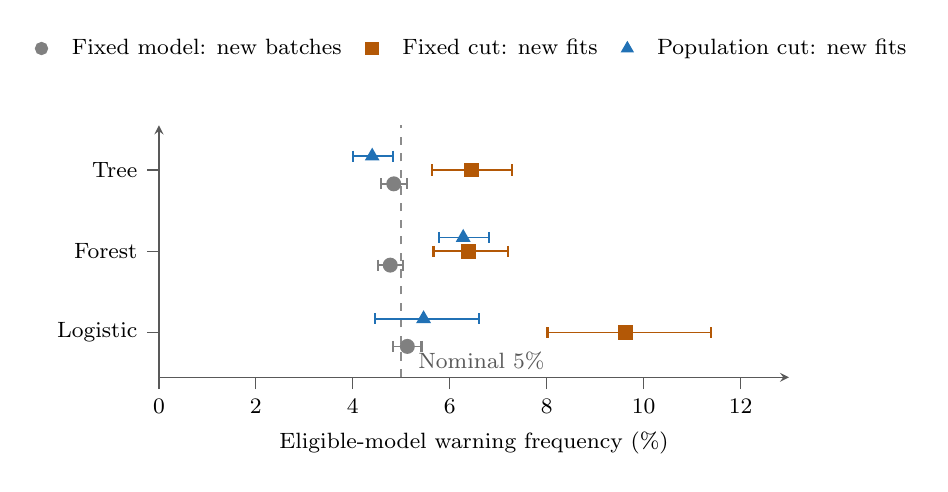
\begin{tikzpicture}
\begin{axis}[auditaxis,width=0.66\textwidth,height=3.2cm,
xmin=0,xmax=13,xtick={0,2,4,6,8,10,12},ymin=0.45,ymax=3.55,
ytick={1,2,3},yticklabels={Logistic,Forest,Tree},
xlabel={Eligible-model warning frequency (\%)},
legend columns=3,legend style={at={(0.5,1.22)},anchor=south}]
\addplot[dashed,color=black!45,line width=0.6pt,forget plot] coordinates {(5,0.45000000000000001) (5,3.5499999999999998)};
\addplot[no marks,color=black!50,line width=0.65pt,forget plot] coordinates {(4.5750000000000002,2.8300000000000001) (5.1100000000000003,2.8300000000000001)};
\addplot[only marks,color=black!50,mark=|,mark size=2pt,forget plot] coordinates {(4.5750000000000002,2.8300000000000001) (5.1100000000000003,2.8300000000000001)};
\addplot[only marks,color=black!50,mark=*,mark size=2.3pt,mark options={fill=black!50,line width=0.8pt},forget plot] coordinates {(4.8450000000000006,2.8300000000000001)};
\addplot[no marks,color=auditorange,line width=0.65pt,forget plot] coordinates {(5.6400000000000006,3) (7.2900625000000012,3)};
\addplot[only marks,color=auditorange,mark=|,mark size=2pt,forget plot] coordinates {(5.6400000000000006,3) (7.2900625000000012,3)};
\addplot[only marks,color=auditorange,mark=square*,mark size=2.3pt,mark options={fill=auditorange,line width=0.8pt},forget plot] coordinates {(6.4450000000000003,3)};
\addplot[no marks,color=auditblue,line width=0.65pt,forget plot] coordinates {(4,3.1699999999999999) (4.832562499999999,3.1699999999999999)};
\addplot[only marks,color=auditblue,mark=|,mark size=2pt,forget plot] coordinates {(4,3.1699999999999999) (4.832562499999999,3.1699999999999999)};
\addplot[only marks,color=auditblue,mark=triangle*,mark size=2.3pt,mark options={fill=auditblue,line width=0.8pt},forget plot] coordinates {(4.4000000000000004,3.1699999999999999)};
\addplot[no marks,color=black!50,line width=0.65pt,forget plot] coordinates {(4.5249375000000009,1.8300000000000001) (5.0351875000000001,1.8300000000000001)};
\addplot[only marks,color=black!50,mark=|,mark size=2pt,forget plot] coordinates {(4.5249375000000009,1.8300000000000001) (5.0351875000000001,1.8300000000000001)};
\addplot[only marks,color=black!50,mark=*,mark size=2.3pt,mark options={fill=black!50,line width=0.8pt},forget plot] coordinates {(4.7725,1.8300000000000001)};
\addplot[no marks,color=auditorange,line width=0.65pt,forget plot] coordinates {(5.6646875000000003,2) (7.2025000000000006,2)};
\addplot[only marks,color=auditorange,mark=|,mark size=2pt,forget plot] coordinates {(5.6646875000000003,2) (7.2025000000000006,2)};
\addplot[only marks,color=auditorange,mark=square*,mark size=2.3pt,mark options={fill=auditorange,line width=0.8pt},forget plot] coordinates {(6.3850000000000007,2)};
\addplot[no marks,color=auditblue,line width=0.65pt,forget plot] coordinates {(5.7800000000000002,2.1699999999999999) (6.8102500000000008,2.1699999999999999)};
\addplot[only marks,color=auditblue,mark=|,mark size=2pt,forget plot] coordinates {(5.7800000000000002,2.1699999999999999) (6.8102500000000008,2.1699999999999999)};
\addplot[only marks,color=auditblue,mark=triangle*,mark size=2.3pt,mark options={fill=auditblue,line width=0.8pt},forget plot] coordinates {(6.2775000000000007,2.1699999999999999)};
\addplot[no marks,color=black!50,line width=0.65pt,forget plot] coordinates {(4.8349375000000014,0.82999999999999996) (5.415,0.82999999999999996)};
\addplot[only marks,color=black!50,mark=|,mark size=2pt,forget plot] coordinates {(4.8349375000000014,0.82999999999999996) (5.415,0.82999999999999996)};
\addplot[only marks,color=black!50,mark=*,mark size=2.3pt,mark options={fill=black!50,line width=0.8pt},forget plot] coordinates {(5.125,0.82999999999999996)};
\addplot[no marks,color=auditorange,line width=0.65pt,forget plot] coordinates {(8.0173125000000027,1) (11.3835,1)};
\addplot[only marks,color=auditorange,mark=|,mark size=2pt,forget plot] coordinates {(8.0173125000000027,1) (11.3835,1)};
\addplot[only marks,color=auditorange,mark=square*,mark size=2.3pt,mark options={fill=auditorange,line width=0.8pt},forget plot] coordinates {(9.6174999999999997,1)};
\addplot[no marks,color=auditblue,line width=0.65pt,forget plot] coordinates {(4.4596250000000008,1.1699999999999999) (6.5975625000000013,1.1699999999999999)};
\addplot[only marks,color=auditblue,mark=|,mark size=2pt,forget plot] coordinates {(4.4596250000000008,1.1699999999999999) (6.5975625000000013,1.1699999999999999)};
\addplot[only marks,color=auditblue,mark=triangle*,mark size=2.3pt,mark options={fill=auditblue,line width=0.8pt},forget plot] coordinates {(5.4600000000000009,1.1699999999999999)};
\addlegendimage{only marks,color=black!50,mark=*,mark options={fill=black!50}}
\addlegendentry{Fixed model: new batches}
\addlegendimage{only marks,color=auditorange,mark=square*,mark options={fill=auditorange}}
\addlegendentry{Fixed cut: new fits}
\addlegendimage{only marks,color=auditblue,mark=triangle*,mark options={fill=auditblue}}
\addlegendentry{Population cut: new fits}
\node[anchor=west,font=\footnotesize,text=black!65] at (axis cs:5.15,0.65) {Nominal 5\%};
\end{axis}
\end{tikzpicture}

\caption{\textbf{Probability-audit warning rates increased on decision-equivalent refits.} SHAP excess used fixed overlap bins and $n=10{,}000$; refits used the same learner family. Each learner had 200 evaluated fits with 200 batches each. Whiskers are 95\% fitted-case bootstrap intervals; population-cut intervals condition on the realized calibration bank. The dashed line marks nominal 5\%.}
\end{figure}
\clearpage
\begin{figure}[!ht]
\centering
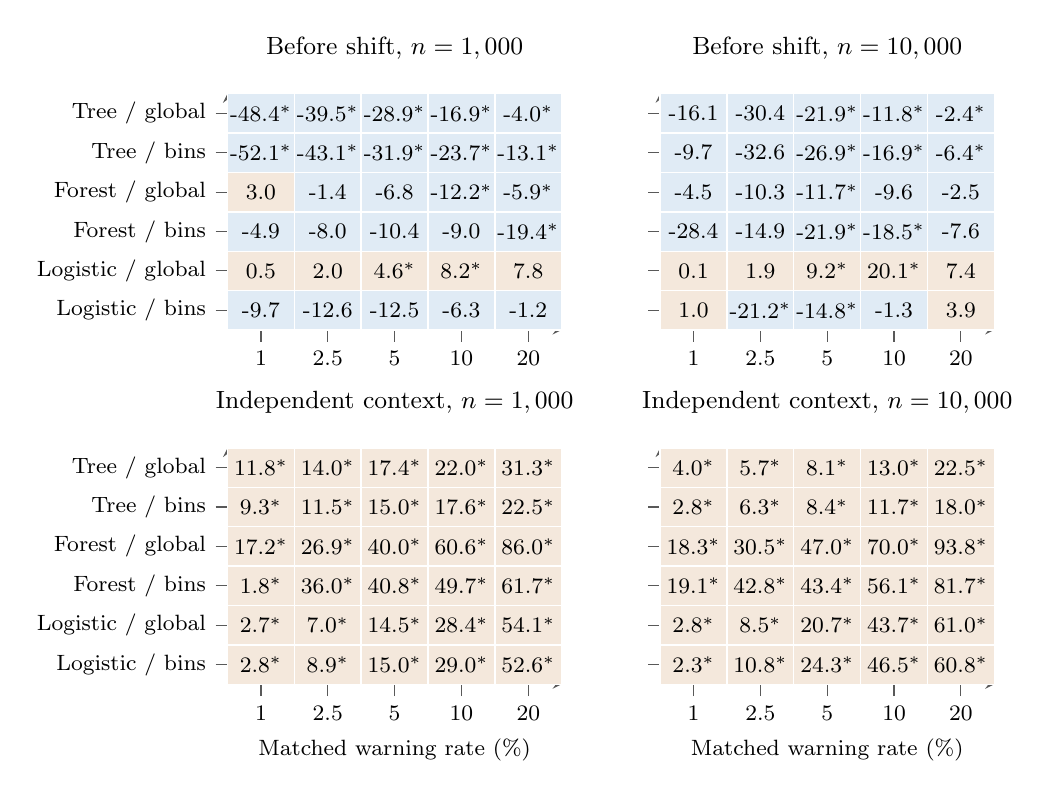
\begin{tikzpicture}
\begin{groupplot}[group style={group size=2 by 2,horizontal sep=1.25cm,vertical sep=1.5cm},
auditaxis,width=0.35\textwidth,height=3.0cm,xmin=0.5,xmax=5.5,ymin=0.5,ymax=6.5,
xtick={1,2,3,4,5},xticklabels={1,2.5,5,10,20},ytick={1,2,3,4,5,6},
xlabel={Matched warning rate (\%)},tick align=outside]
\nextgroupplot[title={Before shift, $n=1,000$},xlabel={},yticklabels={Logistic / bins,Logistic / global,Forest / bins,Forest / global,Tree / bins,Tree / global}]
\path[fill=auditblue!14,draw=white,line width=0.5pt] (axis cs:0.5,5.5) rectangle (axis cs:1.5,6.5);
\node[font=\footnotesize] at (axis cs:1,6) {-48.4$^{*}$};
\path[fill=auditblue!14,draw=white,line width=0.5pt] (axis cs:1.5,5.5) rectangle (axis cs:2.5,6.5);
\node[font=\footnotesize] at (axis cs:2,6) {-39.5$^{*}$};
\path[fill=auditblue!14,draw=white,line width=0.5pt] (axis cs:2.5,5.5) rectangle (axis cs:3.5,6.5);
\node[font=\footnotesize] at (axis cs:3,6) {-28.9$^{*}$};
\path[fill=auditblue!14,draw=white,line width=0.5pt] (axis cs:3.5,5.5) rectangle (axis cs:4.5,6.5);
\node[font=\footnotesize] at (axis cs:4,6) {-16.9$^{*}$};
\path[fill=auditblue!14,draw=white,line width=0.5pt] (axis cs:4.5,5.5) rectangle (axis cs:5.5,6.5);
\node[font=\footnotesize] at (axis cs:5,6) {-4.0$^{*}$};
\path[fill=auditblue!14,draw=white,line width=0.5pt] (axis cs:0.5,4.5) rectangle (axis cs:1.5,5.5);
\node[font=\footnotesize] at (axis cs:1,5) {-52.1$^{*}$};
\path[fill=auditblue!14,draw=white,line width=0.5pt] (axis cs:1.5,4.5) rectangle (axis cs:2.5,5.5);
\node[font=\footnotesize] at (axis cs:2,5) {-43.1$^{*}$};
\path[fill=auditblue!14,draw=white,line width=0.5pt] (axis cs:2.5,4.5) rectangle (axis cs:3.5,5.5);
\node[font=\footnotesize] at (axis cs:3,5) {-31.9$^{*}$};
\path[fill=auditblue!14,draw=white,line width=0.5pt] (axis cs:3.5,4.5) rectangle (axis cs:4.5,5.5);
\node[font=\footnotesize] at (axis cs:4,5) {-23.7$^{*}$};
\path[fill=auditblue!14,draw=white,line width=0.5pt] (axis cs:4.5,4.5) rectangle (axis cs:5.5,5.5);
\node[font=\footnotesize] at (axis cs:5,5) {-13.1$^{*}$};
\path[fill=auditorange!14,draw=white,line width=0.5pt] (axis cs:0.5,3.5) rectangle (axis cs:1.5,4.5);
\node[font=\footnotesize] at (axis cs:1,4) {3.0};
\path[fill=auditblue!14,draw=white,line width=0.5pt] (axis cs:1.5,3.5) rectangle (axis cs:2.5,4.5);
\node[font=\footnotesize] at (axis cs:2,4) {-1.4};
\path[fill=auditblue!14,draw=white,line width=0.5pt] (axis cs:2.5,3.5) rectangle (axis cs:3.5,4.5);
\node[font=\footnotesize] at (axis cs:3,4) {-6.8};
\path[fill=auditblue!14,draw=white,line width=0.5pt] (axis cs:3.5,3.5) rectangle (axis cs:4.5,4.5);
\node[font=\footnotesize] at (axis cs:4,4) {-12.2$^{*}$};
\path[fill=auditblue!14,draw=white,line width=0.5pt] (axis cs:4.5,3.5) rectangle (axis cs:5.5,4.5);
\node[font=\footnotesize] at (axis cs:5,4) {-5.9$^{*}$};
\path[fill=auditblue!14,draw=white,line width=0.5pt] (axis cs:0.5,2.5) rectangle (axis cs:1.5,3.5);
\node[font=\footnotesize] at (axis cs:1,3) {-4.9};
\path[fill=auditblue!14,draw=white,line width=0.5pt] (axis cs:1.5,2.5) rectangle (axis cs:2.5,3.5);
\node[font=\footnotesize] at (axis cs:2,3) {-8.0};
\path[fill=auditblue!14,draw=white,line width=0.5pt] (axis cs:2.5,2.5) rectangle (axis cs:3.5,3.5);
\node[font=\footnotesize] at (axis cs:3,3) {-10.4};
\path[fill=auditblue!14,draw=white,line width=0.5pt] (axis cs:3.5,2.5) rectangle (axis cs:4.5,3.5);
\node[font=\footnotesize] at (axis cs:4,3) {-9.0};
\path[fill=auditblue!14,draw=white,line width=0.5pt] (axis cs:4.5,2.5) rectangle (axis cs:5.5,3.5);
\node[font=\footnotesize] at (axis cs:5,3) {-19.4$^{*}$};
\path[fill=auditorange!14,draw=white,line width=0.5pt] (axis cs:0.5,1.5) rectangle (axis cs:1.5,2.5);
\node[font=\footnotesize] at (axis cs:1,2) {0.5};
\path[fill=auditorange!14,draw=white,line width=0.5pt] (axis cs:1.5,1.5) rectangle (axis cs:2.5,2.5);
\node[font=\footnotesize] at (axis cs:2,2) {2.0};
\path[fill=auditorange!14,draw=white,line width=0.5pt] (axis cs:2.5,1.5) rectangle (axis cs:3.5,2.5);
\node[font=\footnotesize] at (axis cs:3,2) {4.6$^{*}$};
\path[fill=auditorange!14,draw=white,line width=0.5pt] (axis cs:3.5,1.5) rectangle (axis cs:4.5,2.5);
\node[font=\footnotesize] at (axis cs:4,2) {8.2$^{*}$};
\path[fill=auditorange!14,draw=white,line width=0.5pt] (axis cs:4.5,1.5) rectangle (axis cs:5.5,2.5);
\node[font=\footnotesize] at (axis cs:5,2) {7.8};
\path[fill=auditblue!14,draw=white,line width=0.5pt] (axis cs:0.5,0.5) rectangle (axis cs:1.5,1.5);
\node[font=\footnotesize] at (axis cs:1,1) {-9.7};
\path[fill=auditblue!14,draw=white,line width=0.5pt] (axis cs:1.5,0.5) rectangle (axis cs:2.5,1.5);
\node[font=\footnotesize] at (axis cs:2,1) {-12.6};
\path[fill=auditblue!14,draw=white,line width=0.5pt] (axis cs:2.5,0.5) rectangle (axis cs:3.5,1.5);
\node[font=\footnotesize] at (axis cs:3,1) {-12.5};
\path[fill=auditblue!14,draw=white,line width=0.5pt] (axis cs:3.5,0.5) rectangle (axis cs:4.5,1.5);
\node[font=\footnotesize] at (axis cs:4,1) {-6.3};
\path[fill=auditblue!14,draw=white,line width=0.5pt] (axis cs:4.5,0.5) rectangle (axis cs:5.5,1.5);
\node[font=\footnotesize] at (axis cs:5,1) {-1.2};
\nextgroupplot[title={Before shift, $n=10,000$},xlabel={},yticklabels=\empty]
\path[fill=auditblue!14,draw=white,line width=0.5pt] (axis cs:0.5,5.5) rectangle (axis cs:1.5,6.5);
\node[font=\footnotesize] at (axis cs:1,6) {-16.1};
\path[fill=auditblue!14,draw=white,line width=0.5pt] (axis cs:1.5,5.5) rectangle (axis cs:2.5,6.5);
\node[font=\footnotesize] at (axis cs:2,6) {-30.4};
\path[fill=auditblue!14,draw=white,line width=0.5pt] (axis cs:2.5,5.5) rectangle (axis cs:3.5,6.5);
\node[font=\footnotesize] at (axis cs:3,6) {-21.9$^{*}$};
\path[fill=auditblue!14,draw=white,line width=0.5pt] (axis cs:3.5,5.5) rectangle (axis cs:4.5,6.5);
\node[font=\footnotesize] at (axis cs:4,6) {-11.8$^{*}$};
\path[fill=auditblue!14,draw=white,line width=0.5pt] (axis cs:4.5,5.5) rectangle (axis cs:5.5,6.5);
\node[font=\footnotesize] at (axis cs:5,6) {-2.4$^{*}$};
\path[fill=auditblue!14,draw=white,line width=0.5pt] (axis cs:0.5,4.5) rectangle (axis cs:1.5,5.5);
\node[font=\footnotesize] at (axis cs:1,5) {-9.7};
\path[fill=auditblue!14,draw=white,line width=0.5pt] (axis cs:1.5,4.5) rectangle (axis cs:2.5,5.5);
\node[font=\footnotesize] at (axis cs:2,5) {-32.6};
\path[fill=auditblue!14,draw=white,line width=0.5pt] (axis cs:2.5,4.5) rectangle (axis cs:3.5,5.5);
\node[font=\footnotesize] at (axis cs:3,5) {-26.9$^{*}$};
\path[fill=auditblue!14,draw=white,line width=0.5pt] (axis cs:3.5,4.5) rectangle (axis cs:4.5,5.5);
\node[font=\footnotesize] at (axis cs:4,5) {-16.9$^{*}$};
\path[fill=auditblue!14,draw=white,line width=0.5pt] (axis cs:4.5,4.5) rectangle (axis cs:5.5,5.5);
\node[font=\footnotesize] at (axis cs:5,5) {-6.4$^{*}$};
\path[fill=auditblue!14,draw=white,line width=0.5pt] (axis cs:0.5,3.5) rectangle (axis cs:1.5,4.5);
\node[font=\footnotesize] at (axis cs:1,4) {-4.5};
\path[fill=auditblue!14,draw=white,line width=0.5pt] (axis cs:1.5,3.5) rectangle (axis cs:2.5,4.5);
\node[font=\footnotesize] at (axis cs:2,4) {-10.3};
\path[fill=auditblue!14,draw=white,line width=0.5pt] (axis cs:2.5,3.5) rectangle (axis cs:3.5,4.5);
\node[font=\footnotesize] at (axis cs:3,4) {-11.7$^{*}$};
\path[fill=auditblue!14,draw=white,line width=0.5pt] (axis cs:3.5,3.5) rectangle (axis cs:4.5,4.5);
\node[font=\footnotesize] at (axis cs:4,4) {-9.6};
\path[fill=auditblue!14,draw=white,line width=0.5pt] (axis cs:4.5,3.5) rectangle (axis cs:5.5,4.5);
\node[font=\footnotesize] at (axis cs:5,4) {-2.5};
\path[fill=auditblue!14,draw=white,line width=0.5pt] (axis cs:0.5,2.5) rectangle (axis cs:1.5,3.5);
\node[font=\footnotesize] at (axis cs:1,3) {-28.4};
\path[fill=auditblue!14,draw=white,line width=0.5pt] (axis cs:1.5,2.5) rectangle (axis cs:2.5,3.5);
\node[font=\footnotesize] at (axis cs:2,3) {-14.9};
\path[fill=auditblue!14,draw=white,line width=0.5pt] (axis cs:2.5,2.5) rectangle (axis cs:3.5,3.5);
\node[font=\footnotesize] at (axis cs:3,3) {-21.9$^{*}$};
\path[fill=auditblue!14,draw=white,line width=0.5pt] (axis cs:3.5,2.5) rectangle (axis cs:4.5,3.5);
\node[font=\footnotesize] at (axis cs:4,3) {-18.5$^{*}$};
\path[fill=auditblue!14,draw=white,line width=0.5pt] (axis cs:4.5,2.5) rectangle (axis cs:5.5,3.5);
\node[font=\footnotesize] at (axis cs:5,3) {-7.6};
\path[fill=auditorange!14,draw=white,line width=0.5pt] (axis cs:0.5,1.5) rectangle (axis cs:1.5,2.5);
\node[font=\footnotesize] at (axis cs:1,2) {0.1};
\path[fill=auditorange!14,draw=white,line width=0.5pt] (axis cs:1.5,1.5) rectangle (axis cs:2.5,2.5);
\node[font=\footnotesize] at (axis cs:2,2) {1.9};
\path[fill=auditorange!14,draw=white,line width=0.5pt] (axis cs:2.5,1.5) rectangle (axis cs:3.5,2.5);
\node[font=\footnotesize] at (axis cs:3,2) {9.2$^{*}$};
\path[fill=auditorange!14,draw=white,line width=0.5pt] (axis cs:3.5,1.5) rectangle (axis cs:4.5,2.5);
\node[font=\footnotesize] at (axis cs:4,2) {20.1$^{*}$};
\path[fill=auditorange!14,draw=white,line width=0.5pt] (axis cs:4.5,1.5) rectangle (axis cs:5.5,2.5);
\node[font=\footnotesize] at (axis cs:5,2) {7.4};
\path[fill=auditorange!14,draw=white,line width=0.5pt] (axis cs:0.5,0.5) rectangle (axis cs:1.5,1.5);
\node[font=\footnotesize] at (axis cs:1,1) {1.0};
\path[fill=auditblue!14,draw=white,line width=0.5pt] (axis cs:1.5,0.5) rectangle (axis cs:2.5,1.5);
\node[font=\footnotesize] at (axis cs:2,1) {-21.2$^{*}$};
\path[fill=auditblue!14,draw=white,line width=0.5pt] (axis cs:2.5,0.5) rectangle (axis cs:3.5,1.5);
\node[font=\footnotesize] at (axis cs:3,1) {-14.8$^{*}$};
\path[fill=auditblue!14,draw=white,line width=0.5pt] (axis cs:3.5,0.5) rectangle (axis cs:4.5,1.5);
\node[font=\footnotesize] at (axis cs:4,1) {-1.3};
\path[fill=auditorange!14,draw=white,line width=0.5pt] (axis cs:4.5,0.5) rectangle (axis cs:5.5,1.5);
\node[font=\footnotesize] at (axis cs:5,1) {3.9};
\nextgroupplot[title={Independent context, $n=1,000$},yticklabels={Logistic / bins,Logistic / global,Forest / bins,Forest / global,Tree / bins,Tree / global}]
\path[fill=auditorange!14,draw=white,line width=0.5pt] (axis cs:0.5,5.5) rectangle (axis cs:1.5,6.5);
\node[font=\footnotesize] at (axis cs:1,6) {11.8$^{*}$};
\path[fill=auditorange!14,draw=white,line width=0.5pt] (axis cs:1.5,5.5) rectangle (axis cs:2.5,6.5);
\node[font=\footnotesize] at (axis cs:2,6) {14.0$^{*}$};
\path[fill=auditorange!14,draw=white,line width=0.5pt] (axis cs:2.5,5.5) rectangle (axis cs:3.5,6.5);
\node[font=\footnotesize] at (axis cs:3,6) {17.4$^{*}$};
\path[fill=auditorange!14,draw=white,line width=0.5pt] (axis cs:3.5,5.5) rectangle (axis cs:4.5,6.5);
\node[font=\footnotesize] at (axis cs:4,6) {22.0$^{*}$};
\path[fill=auditorange!14,draw=white,line width=0.5pt] (axis cs:4.5,5.5) rectangle (axis cs:5.5,6.5);
\node[font=\footnotesize] at (axis cs:5,6) {31.3$^{*}$};
\path[fill=auditorange!14,draw=white,line width=0.5pt] (axis cs:0.5,4.5) rectangle (axis cs:1.5,5.5);
\node[font=\footnotesize] at (axis cs:1,5) {9.3$^{*}$};
\path[fill=auditorange!14,draw=white,line width=0.5pt] (axis cs:1.5,4.5) rectangle (axis cs:2.5,5.5);
\node[font=\footnotesize] at (axis cs:2,5) {11.5$^{*}$};
\path[fill=auditorange!14,draw=white,line width=0.5pt] (axis cs:2.5,4.5) rectangle (axis cs:3.5,5.5);
\node[font=\footnotesize] at (axis cs:3,5) {15.0$^{*}$};
\path[fill=auditorange!14,draw=white,line width=0.5pt] (axis cs:3.5,4.5) rectangle (axis cs:4.5,5.5);
\node[font=\footnotesize] at (axis cs:4,5) {17.6$^{*}$};
\path[fill=auditorange!14,draw=white,line width=0.5pt] (axis cs:4.5,4.5) rectangle (axis cs:5.5,5.5);
\node[font=\footnotesize] at (axis cs:5,5) {22.5$^{*}$};
\path[fill=auditorange!14,draw=white,line width=0.5pt] (axis cs:0.5,3.5) rectangle (axis cs:1.5,4.5);
\node[font=\footnotesize] at (axis cs:1,4) {17.2$^{*}$};
\path[fill=auditorange!14,draw=white,line width=0.5pt] (axis cs:1.5,3.5) rectangle (axis cs:2.5,4.5);
\node[font=\footnotesize] at (axis cs:2,4) {26.9$^{*}$};
\path[fill=auditorange!14,draw=white,line width=0.5pt] (axis cs:2.5,3.5) rectangle (axis cs:3.5,4.5);
\node[font=\footnotesize] at (axis cs:3,4) {40.0$^{*}$};
\path[fill=auditorange!14,draw=white,line width=0.5pt] (axis cs:3.5,3.5) rectangle (axis cs:4.5,4.5);
\node[font=\footnotesize] at (axis cs:4,4) {60.6$^{*}$};
\path[fill=auditorange!14,draw=white,line width=0.5pt] (axis cs:4.5,3.5) rectangle (axis cs:5.5,4.5);
\node[font=\footnotesize] at (axis cs:5,4) {86.0$^{*}$};
\path[fill=auditorange!14,draw=white,line width=0.5pt] (axis cs:0.5,2.5) rectangle (axis cs:1.5,3.5);
\node[font=\footnotesize] at (axis cs:1,3) {1.8$^{*}$};
\path[fill=auditorange!14,draw=white,line width=0.5pt] (axis cs:1.5,2.5) rectangle (axis cs:2.5,3.5);
\node[font=\footnotesize] at (axis cs:2,3) {36.0$^{*}$};
\path[fill=auditorange!14,draw=white,line width=0.5pt] (axis cs:2.5,2.5) rectangle (axis cs:3.5,3.5);
\node[font=\footnotesize] at (axis cs:3,3) {40.8$^{*}$};
\path[fill=auditorange!14,draw=white,line width=0.5pt] (axis cs:3.5,2.5) rectangle (axis cs:4.5,3.5);
\node[font=\footnotesize] at (axis cs:4,3) {49.7$^{*}$};
\path[fill=auditorange!14,draw=white,line width=0.5pt] (axis cs:4.5,2.5) rectangle (axis cs:5.5,3.5);
\node[font=\footnotesize] at (axis cs:5,3) {61.7$^{*}$};
\path[fill=auditorange!14,draw=white,line width=0.5pt] (axis cs:0.5,1.5) rectangle (axis cs:1.5,2.5);
\node[font=\footnotesize] at (axis cs:1,2) {2.7$^{*}$};
\path[fill=auditorange!14,draw=white,line width=0.5pt] (axis cs:1.5,1.5) rectangle (axis cs:2.5,2.5);
\node[font=\footnotesize] at (axis cs:2,2) {7.0$^{*}$};
\path[fill=auditorange!14,draw=white,line width=0.5pt] (axis cs:2.5,1.5) rectangle (axis cs:3.5,2.5);
\node[font=\footnotesize] at (axis cs:3,2) {14.5$^{*}$};
\path[fill=auditorange!14,draw=white,line width=0.5pt] (axis cs:3.5,1.5) rectangle (axis cs:4.5,2.5);
\node[font=\footnotesize] at (axis cs:4,2) {28.4$^{*}$};
\path[fill=auditorange!14,draw=white,line width=0.5pt] (axis cs:4.5,1.5) rectangle (axis cs:5.5,2.5);
\node[font=\footnotesize] at (axis cs:5,2) {54.1$^{*}$};
\path[fill=auditorange!14,draw=white,line width=0.5pt] (axis cs:0.5,0.5) rectangle (axis cs:1.5,1.5);
\node[font=\footnotesize] at (axis cs:1,1) {2.8$^{*}$};
\path[fill=auditorange!14,draw=white,line width=0.5pt] (axis cs:1.5,0.5) rectangle (axis cs:2.5,1.5);
\node[font=\footnotesize] at (axis cs:2,1) {8.9$^{*}$};
\path[fill=auditorange!14,draw=white,line width=0.5pt] (axis cs:2.5,0.5) rectangle (axis cs:3.5,1.5);
\node[font=\footnotesize] at (axis cs:3,1) {15.0$^{*}$};
\path[fill=auditorange!14,draw=white,line width=0.5pt] (axis cs:3.5,0.5) rectangle (axis cs:4.5,1.5);
\node[font=\footnotesize] at (axis cs:4,1) {29.0$^{*}$};
\path[fill=auditorange!14,draw=white,line width=0.5pt] (axis cs:4.5,0.5) rectangle (axis cs:5.5,1.5);
\node[font=\footnotesize] at (axis cs:5,1) {52.6$^{*}$};
\nextgroupplot[title={Independent context, $n=10,000$},yticklabels=\empty]
\path[fill=auditorange!14,draw=white,line width=0.5pt] (axis cs:0.5,5.5) rectangle (axis cs:1.5,6.5);
\node[font=\footnotesize] at (axis cs:1,6) {4.0$^{*}$};
\path[fill=auditorange!14,draw=white,line width=0.5pt] (axis cs:1.5,5.5) rectangle (axis cs:2.5,6.5);
\node[font=\footnotesize] at (axis cs:2,6) {5.7$^{*}$};
\path[fill=auditorange!14,draw=white,line width=0.5pt] (axis cs:2.5,5.5) rectangle (axis cs:3.5,6.5);
\node[font=\footnotesize] at (axis cs:3,6) {8.1$^{*}$};
\path[fill=auditorange!14,draw=white,line width=0.5pt] (axis cs:3.5,5.5) rectangle (axis cs:4.5,6.5);
\node[font=\footnotesize] at (axis cs:4,6) {13.0$^{*}$};
\path[fill=auditorange!14,draw=white,line width=0.5pt] (axis cs:4.5,5.5) rectangle (axis cs:5.5,6.5);
\node[font=\footnotesize] at (axis cs:5,6) {22.5$^{*}$};
\path[fill=auditorange!14,draw=white,line width=0.5pt] (axis cs:0.5,4.5) rectangle (axis cs:1.5,5.5);
\node[font=\footnotesize] at (axis cs:1,5) {2.8$^{*}$};
\path[fill=auditorange!14,draw=white,line width=0.5pt] (axis cs:1.5,4.5) rectangle (axis cs:2.5,5.5);
\node[font=\footnotesize] at (axis cs:2,5) {6.3$^{*}$};
\path[fill=auditorange!14,draw=white,line width=0.5pt] (axis cs:2.5,4.5) rectangle (axis cs:3.5,5.5);
\node[font=\footnotesize] at (axis cs:3,5) {8.4$^{*}$};
\path[fill=auditorange!14,draw=white,line width=0.5pt] (axis cs:3.5,4.5) rectangle (axis cs:4.5,5.5);
\node[font=\footnotesize] at (axis cs:4,5) {11.7$^{*}$};
\path[fill=auditorange!14,draw=white,line width=0.5pt] (axis cs:4.5,4.5) rectangle (axis cs:5.5,5.5);
\node[font=\footnotesize] at (axis cs:5,5) {18.0$^{*}$};
\path[fill=auditorange!14,draw=white,line width=0.5pt] (axis cs:0.5,3.5) rectangle (axis cs:1.5,4.5);
\node[font=\footnotesize] at (axis cs:1,4) {18.3$^{*}$};
\path[fill=auditorange!14,draw=white,line width=0.5pt] (axis cs:1.5,3.5) rectangle (axis cs:2.5,4.5);
\node[font=\footnotesize] at (axis cs:2,4) {30.5$^{*}$};
\path[fill=auditorange!14,draw=white,line width=0.5pt] (axis cs:2.5,3.5) rectangle (axis cs:3.5,4.5);
\node[font=\footnotesize] at (axis cs:3,4) {47.0$^{*}$};
\path[fill=auditorange!14,draw=white,line width=0.5pt] (axis cs:3.5,3.5) rectangle (axis cs:4.5,4.5);
\node[font=\footnotesize] at (axis cs:4,4) {70.0$^{*}$};
\path[fill=auditorange!14,draw=white,line width=0.5pt] (axis cs:4.5,3.5) rectangle (axis cs:5.5,4.5);
\node[font=\footnotesize] at (axis cs:5,4) {93.8$^{*}$};
\path[fill=auditorange!14,draw=white,line width=0.5pt] (axis cs:0.5,2.5) rectangle (axis cs:1.5,3.5);
\node[font=\footnotesize] at (axis cs:1,3) {19.1$^{*}$};
\path[fill=auditorange!14,draw=white,line width=0.5pt] (axis cs:1.5,2.5) rectangle (axis cs:2.5,3.5);
\node[font=\footnotesize] at (axis cs:2,3) {42.8$^{*}$};
\path[fill=auditorange!14,draw=white,line width=0.5pt] (axis cs:2.5,2.5) rectangle (axis cs:3.5,3.5);
\node[font=\footnotesize] at (axis cs:3,3) {43.4$^{*}$};
\path[fill=auditorange!14,draw=white,line width=0.5pt] (axis cs:3.5,2.5) rectangle (axis cs:4.5,3.5);
\node[font=\footnotesize] at (axis cs:4,3) {56.1$^{*}$};
\path[fill=auditorange!14,draw=white,line width=0.5pt] (axis cs:4.5,2.5) rectangle (axis cs:5.5,3.5);
\node[font=\footnotesize] at (axis cs:5,3) {81.7$^{*}$};
\path[fill=auditorange!14,draw=white,line width=0.5pt] (axis cs:0.5,1.5) rectangle (axis cs:1.5,2.5);
\node[font=\footnotesize] at (axis cs:1,2) {2.8$^{*}$};
\path[fill=auditorange!14,draw=white,line width=0.5pt] (axis cs:1.5,1.5) rectangle (axis cs:2.5,2.5);
\node[font=\footnotesize] at (axis cs:2,2) {8.5$^{*}$};
\path[fill=auditorange!14,draw=white,line width=0.5pt] (axis cs:2.5,1.5) rectangle (axis cs:3.5,2.5);
\node[font=\footnotesize] at (axis cs:3,2) {20.7$^{*}$};
\path[fill=auditorange!14,draw=white,line width=0.5pt] (axis cs:3.5,1.5) rectangle (axis cs:4.5,2.5);
\node[font=\footnotesize] at (axis cs:4,2) {43.7$^{*}$};
\path[fill=auditorange!14,draw=white,line width=0.5pt] (axis cs:4.5,1.5) rectangle (axis cs:5.5,2.5);
\node[font=\footnotesize] at (axis cs:5,2) {61.0$^{*}$};
\path[fill=auditorange!14,draw=white,line width=0.5pt] (axis cs:0.5,0.5) rectangle (axis cs:1.5,1.5);
\node[font=\footnotesize] at (axis cs:1,1) {2.3$^{*}$};
\path[fill=auditorange!14,draw=white,line width=0.5pt] (axis cs:1.5,0.5) rectangle (axis cs:2.5,1.5);
\node[font=\footnotesize] at (axis cs:2,1) {10.8$^{*}$};
\path[fill=auditorange!14,draw=white,line width=0.5pt] (axis cs:2.5,0.5) rectangle (axis cs:3.5,1.5);
\node[font=\footnotesize] at (axis cs:3,1) {24.3$^{*}$};
\path[fill=auditorange!14,draw=white,line width=0.5pt] (axis cs:3.5,0.5) rectangle (axis cs:4.5,1.5);
\node[font=\footnotesize] at (axis cs:4,1) {46.5$^{*}$};
\path[fill=auditorange!14,draw=white,line width=0.5pt] (axis cs:4.5,0.5) rectangle (axis cs:5.5,1.5);
\node[font=\footnotesize] at (axis cs:5,1) {60.8$^{*}$};
\end{groupplot}
\end{tikzpicture}

\caption{\textbf{Localization differences depend on learner, warning rate, and context law.} All 120 cells show flip-minus-SHAP localization differences in percentage points across two sizes, two partitions, five matched warning rates, and two laws. Blue/negative favors SHAP; orange/positive favors flip. An asterisk marks a pointwise 95\% paired-bootstrap interval excluding zero; these intervals are not multiplicity-adjusted. Fixed bins use target-law knowledge. Matching was retrospective.}
\end{figure}
\clearpage
\begin{figure}[!ht]
\centering
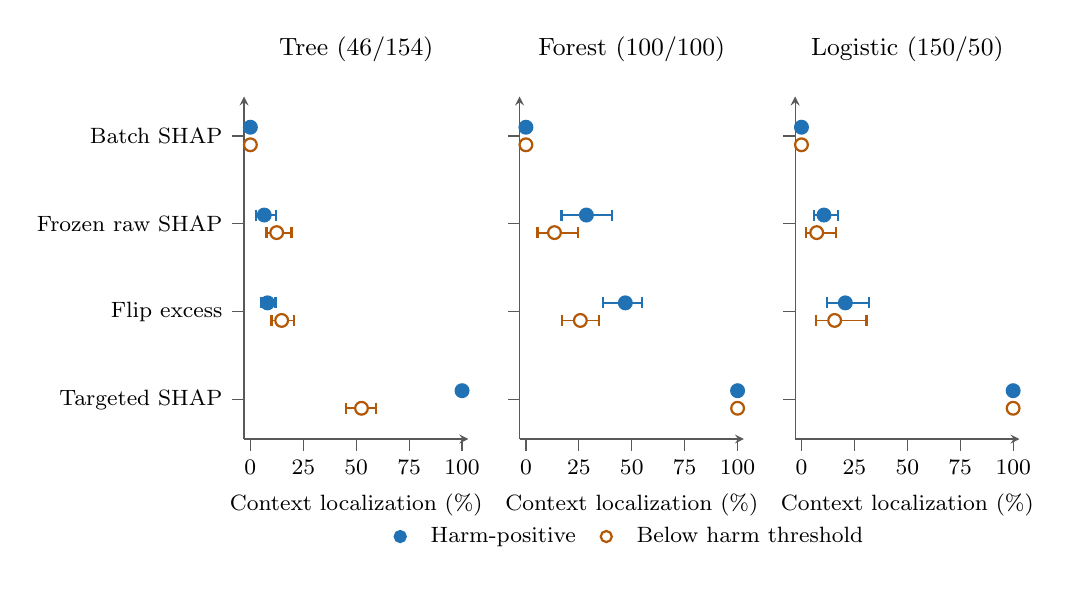
\begin{tikzpicture}
\begin{groupplot}[group style={group size=3 by 1,horizontal sep=0.65cm},
auditaxis,width=0.235\textwidth,height=4.35cm,xmin=-3,xmax=103,
xtick={0,25,50,75,100},ymin=0.55,ymax=4.45,ytick={1,2,3,4},
xlabel={Context localization (\%)}]
\nextgroupplot[title={Tree (46/154)},yticklabels={Targeted SHAP,Flip excess,Frozen raw SHAP,Batch SHAP},legend to name=specificitylegend,legend columns=2]
\addplot[no marks,color=auditblue,line width=0.65pt,forget plot] coordinates {(0,4.0999999999999996) (0,4.0999999999999996)};
\addplot[only marks,color=auditblue,mark=|,mark size=2pt,forget plot] coordinates {(0,4.0999999999999996) (0,4.0999999999999996)};
\addplot[only marks,color=auditblue,mark=*,mark size=2.3pt,mark options={fill=auditblue,line width=0.8pt},forget plot] coordinates {(0,4.0999999999999996)};
\addplot[no marks,color=auditorange,line width=0.65pt,forget plot] coordinates {(0,3.8999999999999999) (0,3.8999999999999999)};
\addplot[only marks,color=auditorange,mark=|,mark size=2pt,forget plot] coordinates {(0,3.8999999999999999) (0,3.8999999999999999)};
\addplot[only marks,color=auditorange,mark=*,mark size=2.3pt,mark options={fill=white,line width=0.8pt},forget plot] coordinates {(0,3.8999999999999999)};
\addplot[no marks,color=auditblue,line width=0.65pt,forget plot] coordinates {(2.6878997077571647,3.1000000000000001) (11.956541651852161,3.1000000000000001)};
\addplot[only marks,color=auditblue,mark=|,mark size=2pt,forget plot] coordinates {(2.6878997077571647,3.1000000000000001) (11.956541651852161,3.1000000000000001)};
\addplot[only marks,color=auditblue,mark=*,mark size=2.3pt,mark options={fill=auditblue,line width=0.8pt},forget plot] coordinates {(6.5500566350091489,3.1000000000000001)};
\addplot[no marks,color=auditorange,line width=0.65pt,forget plot] coordinates {(7.6558999335633953,2.8999999999999999) (19.44751926618299,2.8999999999999999)};
\addplot[only marks,color=auditorange,mark=|,mark size=2pt,forget plot] coordinates {(7.6558999335633953,2.8999999999999999) (19.44751926618299,2.8999999999999999)};
\addplot[only marks,color=auditorange,mark=*,mark size=2.3pt,mark options={fill=white,line width=0.8pt},forget plot] coordinates {(12.423652499804804,2.8999999999999999)};
\addplot[no marks,color=auditblue,line width=0.65pt,forget plot] coordinates {(5.2494485770797352,2.1000000000000001) (11.838578925318085,2.1000000000000001)};
\addplot[only marks,color=auditblue,mark=|,mark size=2pt,forget plot] coordinates {(5.2494485770797352,2.1000000000000001) (11.838578925318085,2.1000000000000001)};
\addplot[only marks,color=auditblue,mark=*,mark size=2.3pt,mark options={fill=auditblue,line width=0.8pt},forget plot] coordinates {(8.0818577075098812,2.1000000000000001)};
\addplot[no marks,color=auditorange,line width=0.65pt,forget plot] coordinates {(9.9609811332251166,1.8999999999999999) (20.659590780619023,1.8999999999999999)};
\addplot[only marks,color=auditorange,mark=|,mark size=2pt,forget plot] coordinates {(9.9609811332251166,1.8999999999999999) (20.659590780619023,1.8999999999999999)};
\addplot[only marks,color=auditorange,mark=*,mark size=2.3pt,mark options={fill=white,line width=0.8pt},forget plot] coordinates {(14.777119244391972,1.8999999999999999)};
\addplot[no marks,color=auditblue,line width=0.65pt,forget plot] coordinates {(100,1.1000000000000001) (100,1.1000000000000001)};
\addplot[only marks,color=auditblue,mark=|,mark size=2pt,forget plot] coordinates {(100,1.1000000000000001) (100,1.1000000000000001)};
\addplot[only marks,color=auditblue,mark=*,mark size=2.3pt,mark options={fill=auditblue,line width=0.8pt},forget plot] coordinates {(100,1.1000000000000001)};
\addplot[no marks,color=auditorange,line width=0.65pt,forget plot] coordinates {(45.117085754357852,0.90000000000000002) (59.209059304703473,0.90000000000000002)};
\addplot[only marks,color=auditorange,mark=|,mark size=2pt,forget plot] coordinates {(45.117085754357852,0.90000000000000002) (59.209059304703473,0.90000000000000002)};
\addplot[only marks,color=auditorange,mark=*,mark size=2.3pt,mark options={fill=white,line width=0.8pt},forget plot] coordinates {(52.5,0.90000000000000002)};
\addlegendimage{only marks,color=auditblue,mark=*,mark options={fill=auditblue}}
\addlegendentry{Harm-positive}
\addlegendimage{only marks,color=auditorange,mark=*,mark options={fill=white}}
\addlegendentry{Below harm threshold}
\nextgroupplot[title={Forest (100/100)},yticklabels=\empty]
\addplot[no marks,color=auditblue,line width=0.65pt,forget plot] coordinates {(0,4.0999999999999996) (0,4.0999999999999996)};
\addplot[only marks,color=auditblue,mark=|,mark size=2pt,forget plot] coordinates {(0,4.0999999999999996) (0,4.0999999999999996)};
\addplot[only marks,color=auditblue,mark=*,mark size=2.3pt,mark options={fill=auditblue,line width=0.8pt},forget plot] coordinates {(0,4.0999999999999996)};
\addplot[no marks,color=auditorange,line width=0.65pt,forget plot] coordinates {(0,3.8999999999999999) (0,3.8999999999999999)};
\addplot[only marks,color=auditorange,mark=|,mark size=2pt,forget plot] coordinates {(0,3.8999999999999999) (0,3.8999999999999999)};
\addplot[only marks,color=auditorange,mark=*,mark size=2.3pt,mark options={fill=white,line width=0.8pt},forget plot] coordinates {(0,3.8999999999999999)};
\addplot[no marks,color=auditblue,line width=0.65pt,forget plot] coordinates {(16.854832034982266,3.1000000000000001) (40.753642386894285,3.1000000000000001)};
\addplot[only marks,color=auditblue,mark=|,mark size=2pt,forget plot] coordinates {(16.854832034982266,3.1000000000000001) (40.753642386894285,3.1000000000000001)};
\addplot[only marks,color=auditblue,mark=*,mark size=2.3pt,mark options={fill=auditblue,line width=0.8pt},forget plot] coordinates {(28.580844155844154,3.1000000000000001)};
\addplot[no marks,color=auditorange,line width=0.65pt,forget plot] coordinates {(5.4967969367851772,2.8999999999999999) (24.595630466835043,2.8999999999999999)};
\addplot[only marks,color=auditorange,mark=|,mark size=2pt,forget plot] coordinates {(5.4967969367851772,2.8999999999999999) (24.595630466835043,2.8999999999999999)};
\addplot[only marks,color=auditorange,mark=*,mark size=2.3pt,mark options={fill=white,line width=0.8pt},forget plot] coordinates {(13.4937012987013,2.8999999999999999)};
\addplot[no marks,color=auditblue,line width=0.65pt,forget plot] coordinates {(36.240990788294638,2.1000000000000001) (54.931050892059552,2.1000000000000001)};
\addplot[only marks,color=auditblue,mark=|,mark size=2pt,forget plot] coordinates {(36.240990788294638,2.1000000000000001) (54.931050892059552,2.1000000000000001)};
\addplot[only marks,color=auditblue,mark=*,mark size=2.3pt,mark options={fill=auditblue,line width=0.8pt},forget plot] coordinates {(46.958367427222655,2.1000000000000001)};
\addplot[no marks,color=auditorange,line width=0.65pt,forget plot] coordinates {(17.138138655088408,1.8999999999999999) (34.641582679126003,1.8999999999999999)};
\addplot[only marks,color=auditorange,mark=|,mark size=2pt,forget plot] coordinates {(17.138138655088408,1.8999999999999999) (34.641582679126003,1.8999999999999999)};
\addplot[only marks,color=auditorange,mark=*,mark size=2.3pt,mark options={fill=white,line width=0.8pt},forget plot] coordinates {(25.715106215578288,1.8999999999999999)};
\addplot[no marks,color=auditblue,line width=0.65pt,forget plot] coordinates {(100,1.1000000000000001) (100,1.1000000000000001)};
\addplot[only marks,color=auditblue,mark=|,mark size=2pt,forget plot] coordinates {(100,1.1000000000000001) (100,1.1000000000000001)};
\addplot[only marks,color=auditblue,mark=*,mark size=2.3pt,mark options={fill=auditblue,line width=0.8pt},forget plot] coordinates {(100,1.1000000000000001)};
\addplot[no marks,color=auditorange,line width=0.65pt,forget plot] coordinates {(100,0.90000000000000002) (100,0.90000000000000002)};
\addplot[only marks,color=auditorange,mark=|,mark size=2pt,forget plot] coordinates {(100,0.90000000000000002) (100,0.90000000000000002)};
\addplot[only marks,color=auditorange,mark=*,mark size=2.3pt,mark options={fill=white,line width=0.8pt},forget plot] coordinates {(100,0.90000000000000002)};
\nextgroupplot[title={Logistic (150/50)},yticklabels=\empty]
\addplot[no marks,color=auditblue,line width=0.65pt,forget plot] coordinates {(0,4.0999999999999996) (0,4.0999999999999996)};
\addplot[only marks,color=auditblue,mark=|,mark size=2pt,forget plot] coordinates {(0,4.0999999999999996) (0,4.0999999999999996)};
\addplot[only marks,color=auditblue,mark=*,mark size=2.3pt,mark options={fill=auditblue,line width=0.8pt},forget plot] coordinates {(0,4.0999999999999996)};
\addplot[no marks,color=auditorange,line width=0.65pt,forget plot] coordinates {(0,3.8999999999999999) (0,3.8999999999999999)};
\addplot[only marks,color=auditorange,mark=|,mark size=2pt,forget plot] coordinates {(0,3.8999999999999999) (0,3.8999999999999999)};
\addplot[only marks,color=auditorange,mark=*,mark size=2.3pt,mark options={fill=white,line width=0.8pt},forget plot] coordinates {(0,3.8999999999999999)};
\addplot[no marks,color=auditblue,line width=0.65pt,forget plot] coordinates {(5.8558526711016228,3.1000000000000001) (17.100600013752132,3.1000000000000001)};
\addplot[only marks,color=auditblue,mark=|,mark size=2pt,forget plot] coordinates {(5.8558526711016228,3.1000000000000001) (17.100600013752132,3.1000000000000001)};
\addplot[only marks,color=auditblue,mark=*,mark size=2.3pt,mark options={fill=auditblue,line width=0.8pt},forget plot] coordinates {(10.624523007856341,3.1000000000000001)};
\addplot[no marks,color=auditorange,line width=0.65pt,forget plot] coordinates {(2.0572656786118704,2.8999999999999999) (16.465942115922232,2.8999999999999999)};
\addplot[only marks,color=auditorange,mark=|,mark size=2pt,forget plot] coordinates {(2.0572656786118704,2.8999999999999999) (16.465942115922232,2.8999999999999999)};
\addplot[only marks,color=auditorange,mark=*,mark size=2.3pt,mark options={fill=white,line width=0.8pt},forget plot] coordinates {(7.1949494949494959,2.8999999999999999)};
\addplot[no marks,color=auditblue,line width=0.65pt,forget plot] coordinates {(12.198390682128499,2.1000000000000001) (31.780801179082879,2.1000000000000001)};
\addplot[only marks,color=auditblue,mark=|,mark size=2pt,forget plot] coordinates {(12.198390682128499,2.1000000000000001) (31.780801179082879,2.1000000000000001)};
\addplot[only marks,color=auditblue,mark=*,mark size=2.3pt,mark options={fill=auditblue,line width=0.8pt},forget plot] coordinates {(20.716099290780139,2.1000000000000001)};
\addplot[no marks,color=auditorange,line width=0.65pt,forget plot] coordinates {(6.9961743262162255,1.8999999999999999) (30.69647599013437,1.8999999999999999)};
\addplot[only marks,color=auditorange,mark=|,mark size=2pt,forget plot] coordinates {(6.9961743262162255,1.8999999999999999) (30.69647599013437,1.8999999999999999)};
\addplot[only marks,color=auditorange,mark=*,mark size=2.3pt,mark options={fill=white,line width=0.8pt},forget plot] coordinates {(15.678404255319148,1.8999999999999999)};
\addplot[no marks,color=auditblue,line width=0.65pt,forget plot] coordinates {(100,1.1000000000000001) (100,1.1000000000000001)};
\addplot[only marks,color=auditblue,mark=|,mark size=2pt,forget plot] coordinates {(100,1.1000000000000001) (100,1.1000000000000001)};
\addplot[only marks,color=auditblue,mark=*,mark size=2.3pt,mark options={fill=auditblue,line width=0.8pt},forget plot] coordinates {(100,1.1000000000000001)};
\addplot[no marks,color=auditorange,line width=0.65pt,forget plot] coordinates {(100,0.90000000000000002) (100,0.90000000000000002)};
\addplot[only marks,color=auditorange,mark=|,mark size=2pt,forget plot] coordinates {(100,0.90000000000000002) (100,0.90000000000000002)};
\addplot[only marks,color=auditorange,mark=*,mark size=2.3pt,mark options={fill=white,line width=0.8pt},forget plot] coordinates {(100,0.90000000000000002)};
\end{groupplot}
\node[anchor=north] at ([yshift=-0.85cm]group c2r1.south) {\pgfplotslegendfromname{specificitylegend}};
\end{tikzpicture}

\caption{\textbf{Post-shift localization did not consistently separate the harm groups.} Selected score designs used global population ranks at matched 5\% empirical eligible-model warnings and $n=10{,}000$. Filled/hollow points denote $H_i\geq0.05$/$H_i<0.05$; panel counts follow that order. Whiskers are pointwise 95\% paired-bootstrap intervals. Batch SHAP is normalized; frozen raw SHAP changes both background and normalization. Targeted SHAP knows $C$; complete ablations accompany the numerical data.}
\end{figure}
\clearpage
\begin{figure}[!ht]
\centering
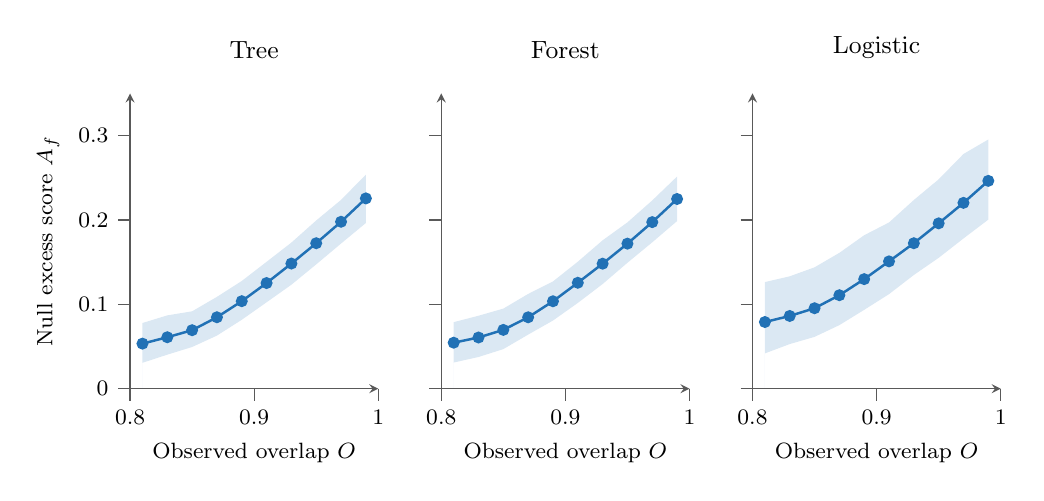
\begin{tikzpicture}
\begin{groupplot}[group style={group size=3 by 1,horizontal sep=0.8cm},
auditaxis,width=0.26\textwidth,height=3.75cm,xmin=0.8,xmax=1,ymin=0,ymax=0.35,
xtick={0.8,0.9,1},ytick={0,0.1,0.2,0.3},xlabel={Observed overlap $O$}]
\nextgroupplot[title={Tree},ylabel={Null excess score $A_f$}]
\addplot[draw=none,fill=auditblue,fill opacity=0.16] coordinates {(0.81000000000000005,0.030695853390183894) (0.83000000000000007,0.040345039964228127) (0.85000000000000009,0.049426382261028148) (0.87,0.062944288488821151) (0.89000000000000001,0.081681099642497285) (0.91000000000000003,0.1024207277813456) (0.93000000000000005,0.12326345541572085) (0.94999999999999996,0.14736329085839944) (0.96999999999999997,0.17206279663949209) (0.98999999999999999,0.19641280650593679) (0.98999999999999999,0.25376345048495585) (0.96999999999999997,0.22382694595363373) (0.94999999999999996,0.19945198455272989) (0.93000000000000005,0.17324630891956222) (0.91000000000000003,0.1504103098645681) (0.89000000000000001,0.12769617210129416) (0.87,0.10887630037404279) (0.85000000000000009,0.091740641883218912) (0.83000000000000007,0.086938263590634723) (0.81000000000000005,0.07790002289478587)} \closedcycle;
\addplot[color=auditblue,mark=*,mark size=1.7pt,line width=0.9pt] coordinates {(0.81000000000000005,0.053433104592902306) (0.83000000000000007,0.061004086535639594) (0.85000000000000009,0.069352136094997185) (0.87,0.084691742111262971) (0.89000000000000001,0.10374980682054996) (0.91000000000000003,0.12525121151043733) (0.93000000000000005,0.14836021942738303) (0.94999999999999996,0.17246112658829396) (0.96999999999999997,0.19787859453296019) (0.98999999999999999,0.22559250661004104)};
\nextgroupplot[title={Forest},yticklabels=\empty]
\addplot[draw=none,fill=auditblue,fill opacity=0.16] coordinates {(0.81000000000000005,0.031006751203862679) (0.83000000000000007,0.037576692758860095) (0.85000000000000009,0.046931641026983176) (0.87,0.064113433886885354) (0.89000000000000001,0.080798747937904092) (0.91000000000000003,0.10164759912673649) (0.93000000000000005,0.12406386720975801) (0.94999999999999996,0.14925955670488977) (0.96999999999999997,0.17354297835259266) (0.98999999999999999,0.19871235073032825) (0.98999999999999999,0.25154216678122315) (0.96999999999999997,0.22322361321063022) (0.94999999999999996,0.19717724598464878) (0.93000000000000005,0.1759125767175545) (0.91000000000000003,0.1505430062167403) (0.89000000000000001,0.12714874732839068) (0.87,0.11234830243881624) (0.85000000000000009,0.094955304556422926) (0.83000000000000007,0.086511468773126127) (0.81000000000000005,0.078889145283800421)} \closedcycle;
\addplot[color=auditblue,mark=*,mark size=1.7pt,line width=0.9pt] coordinates {(0.81000000000000005,0.054539962686251206) (0.83000000000000007,0.060698654820590156) (0.85000000000000009,0.069723547892054108) (0.87,0.084664464272734344) (0.89000000000000001,0.10365712499597696) (0.91000000000000003,0.12557946674634438) (0.93000000000000005,0.148200809393703) (0.94999999999999996,0.17196024960642006) (0.96999999999999997,0.1974664429866089) (0.98999999999999999,0.22488328148856698)};
\nextgroupplot[title={Logistic},yticklabels=\empty]
\addplot[draw=none,fill=auditblue,fill opacity=0.16] coordinates {(0.81000000000000005,0.041853639828600707) (0.83000000000000007,0.052901582189324184) (0.85000000000000009,0.061433298274001825) (0.87,0.075362889453188669) (0.89000000000000001,0.093473995951535466) (0.91000000000000003,0.11209310862293888) (0.93000000000000005,0.13479101918118103) (0.94999999999999996,0.15511561926882506) (0.96999999999999997,0.17808638033028973) (0.98999999999999999,0.20042079059762222) (0.98999999999999999,0.29543634569524319) (0.96999999999999997,0.27825018507948923) (0.94999999999999996,0.24819181117111253) (0.93000000000000005,0.22371425254875324) (0.91000000000000003,0.19707706283494861) (0.89000000000000001,0.18193784026753532) (0.87,0.16104871997597864) (0.85000000000000009,0.14389717029974661) (0.83000000000000007,0.13322780836981943) (0.81000000000000005,0.12640973152007348)} \closedcycle;
\addplot[color=auditblue,mark=*,mark size=1.7pt,line width=0.9pt] coordinates {(0.81000000000000005,0.079043366980431157) (0.83000000000000007,0.086227249687442165) (0.85000000000000009,0.095399409754082606) (0.87,0.11082980779563638) (0.89000000000000001,0.12989734722690105) (0.91000000000000003,0.15094798434065876) (0.93000000000000005,0.17245589709699818) (0.94999999999999996,0.19600929282633728) (0.96999999999999997,0.22029974677183359) (0.98999999999999999,0.246365371145263)};
\end{groupplot}
\end{tikzpicture}

\caption{\textbf{Null attribution excess increased with mechanism overlap in every learner.} Curves average within-interval means over 200 references at $n=10{,}000$. Shading spans the 2.5th--97.5th percentiles across those reference means; it is not a confidence band. The ten plotted overlap intervals summarize curves; calibration instead uses the stated global or three-bin rule.}
\end{figure}
\clearpage
\begin{figure}[!ht]
\centering
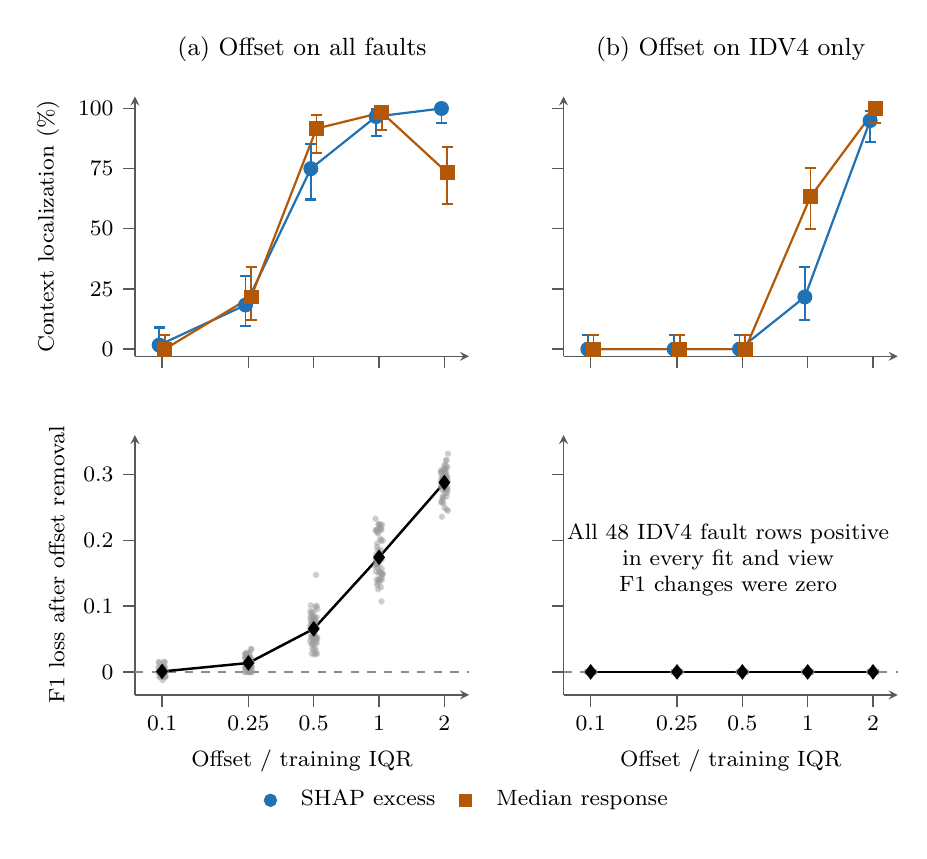
\begin{tikzpicture}
\begin{groupplot}[group style={group size=2 by 2,horizontal sep=1.2cm,vertical sep=1.0cm},
auditaxis,width=0.35\textwidth,height=3.3cm,xmode=log,log basis x=2,
xmin=0.075,xmax=2.6,xtick={0.1,0.25,0.5,1,2},xticklabels={0.1,0.25,0.5,1,2}]
\nextgroupplot[title={(a) Offset on all faults},ymin=-3,ymax=105,ytick={0,25,50,75,100},xticklabels=\empty,ylabel={Context localization (\%)},legend to name=doselegend,legend columns=2]
\addplot[color=auditblue,no marks,forget plot] coordinates {(0.097000000000000003,1.6666666666666667) (0.24249999999999999,18.333333333333332) (0.48499999999999999,75) (0.96999999999999997,96.666666666666671) (1.9399999999999999,100)};
\addlegendimage{only marks,color=auditblue,mark=*,mark options={fill=auditblue}}
\addlegendentry{SHAP excess}
\addplot[no marks,color=auditblue,line width=0.65pt,forget plot] coordinates {(0.097000000000000003,0.042187445234200913) (0.097000000000000003,8.9399050057486988)};
\addplot[only marks,color=auditblue,mark=-,mark size=2pt,forget plot] coordinates {(0.097000000000000003,0.042187445234200913) (0.097000000000000003,8.9399050057486988)};
\addplot[only marks,color=auditblue,mark=*,mark size=2.3pt,mark options={fill=auditblue,line width=0.8pt},forget plot] coordinates {(0.097000000000000003,1.6666666666666667)};
\addplot[no marks,color=auditblue,line width=0.65pt,forget plot] coordinates {(0.24249999999999999,9.5235822916563801) (0.24249999999999999,30.439605474077624)};
\addplot[only marks,color=auditblue,mark=-,mark size=2pt,forget plot] coordinates {(0.24249999999999999,9.5235822916563801) (0.24249999999999999,30.439605474077624)};
\addplot[only marks,color=auditblue,mark=*,mark size=2.3pt,mark options={fill=auditblue,line width=0.8pt},forget plot] coordinates {(0.24249999999999999,18.333333333333332)};
\addplot[no marks,color=auditblue,line width=0.65pt,forget plot] coordinates {(0.48499999999999999,62.140364452045574) (0.48499999999999999,85.281392620099638)};
\addplot[only marks,color=auditblue,mark=-,mark size=2pt,forget plot] coordinates {(0.48499999999999999,62.140364452045574) (0.48499999999999999,85.281392620099638)};
\addplot[only marks,color=auditblue,mark=*,mark size=2.3pt,mark options={fill=auditblue,line width=0.8pt},forget plot] coordinates {(0.48499999999999999,75)};
\addplot[no marks,color=auditblue,line width=0.65pt,forget plot] coordinates {(0.96999999999999997,88.471895558074834) (0.96999999999999997,99.593737535790652)};
\addplot[only marks,color=auditblue,mark=-,mark size=2pt,forget plot] coordinates {(0.96999999999999997,88.471895558074834) (0.96999999999999997,99.593737535790652)};
\addplot[only marks,color=auditblue,mark=*,mark size=2.3pt,mark options={fill=auditblue,line width=0.8pt},forget plot] coordinates {(0.96999999999999997,96.666666666666671)};
\addplot[no marks,color=auditblue,line width=0.65pt,forget plot] coordinates {(1.9399999999999999,94.037050771383306) (1.9399999999999999,100)};
\addplot[only marks,color=auditblue,mark=-,mark size=2pt,forget plot] coordinates {(1.9399999999999999,94.037050771383306) (1.9399999999999999,100)};
\addplot[only marks,color=auditblue,mark=*,mark size=2.3pt,mark options={fill=auditblue,line width=0.8pt},forget plot] coordinates {(1.9399999999999999,100)};
\addplot[color=auditorange,no marks,forget plot] coordinates {(0.10300000000000001,0) (0.25750000000000001,21.666666666666668) (0.51500000000000001,91.666666666666671) (1.03,98.333333333333329) (2.0600000000000001,73.333333333333329)};
\addlegendimage{only marks,color=auditorange,mark=square*,mark options={fill=auditorange}}
\addlegendentry{Median response}
\addplot[no marks,color=auditorange,line width=0.65pt,forget plot] coordinates {(0.10300000000000001,0) (0.10300000000000001,5.9629492286166919)};
\addplot[only marks,color=auditorange,mark=-,mark size=2pt,forget plot] coordinates {(0.10300000000000001,0) (0.10300000000000001,5.9629492286166919)};
\addplot[only marks,color=auditorange,mark=square*,mark size=2.3pt,mark options={fill=auditorange,line width=0.8pt},forget plot] coordinates {(0.10300000000000001,0)};
\addplot[no marks,color=auditorange,line width=0.65pt,forget plot] coordinates {(0.25750000000000001,12.071602446269679) (0.25750000000000001,34.195617873465253)};
\addplot[only marks,color=auditorange,mark=-,mark size=2pt,forget plot] coordinates {(0.25750000000000001,12.071602446269679) (0.25750000000000001,34.195617873465253)};
\addplot[only marks,color=auditorange,mark=square*,mark size=2.3pt,mark options={fill=auditorange,line width=0.8pt},forget plot] coordinates {(0.25750000000000001,21.666666666666668)};
\addplot[no marks,color=auditorange,line width=0.65pt,forget plot] coordinates {(0.51500000000000001,81.614221662341421) (0.51500000000000001,97.238668966257364)};
\addplot[only marks,color=auditorange,mark=-,mark size=2pt,forget plot] coordinates {(0.51500000000000001,81.614221662341421) (0.51500000000000001,97.238668966257364)};
\addplot[only marks,color=auditorange,mark=square*,mark size=2.3pt,mark options={fill=auditorange,line width=0.8pt},forget plot] coordinates {(0.51500000000000001,91.666666666666671)};
\addplot[no marks,color=auditorange,line width=0.65pt,forget plot] coordinates {(1.03,91.060094994251301) (1.03,99.957812554765795)};
\addplot[only marks,color=auditorange,mark=-,mark size=2pt,forget plot] coordinates {(1.03,91.060094994251301) (1.03,99.957812554765795)};
\addplot[only marks,color=auditorange,mark=square*,mark size=2.3pt,mark options={fill=auditorange,line width=0.8pt},forget plot] coordinates {(1.03,98.333333333333329)};
\addplot[no marks,color=auditorange,line width=0.65pt,forget plot] coordinates {(2.0600000000000001,60.338965997450444) (2.0600000000000001,83.925354840958462)};
\addplot[only marks,color=auditorange,mark=-,mark size=2pt,forget plot] coordinates {(2.0600000000000001,60.338965997450444) (2.0600000000000001,83.925354840958462)};
\addplot[only marks,color=auditorange,mark=square*,mark size=2.3pt,mark options={fill=auditorange,line width=0.8pt},forget plot] coordinates {(2.0600000000000001,73.333333333333329)};
\nextgroupplot[title={(b) Offset on IDV4 only},ymin=-3,ymax=105,ytick={0,25,50,75,100},xticklabels=\empty,yticklabels=\empty]
\addplot[color=auditblue,no marks,forget plot] coordinates {(0.097000000000000003,0) (0.24249999999999999,0) (0.48499999999999999,0) (0.96999999999999997,21.666666666666668) (1.9399999999999999,95)};
\addplot[no marks,color=auditblue,line width=0.65pt,forget plot] coordinates {(0.097000000000000003,0) (0.097000000000000003,5.9629492286166919)};
\addplot[only marks,color=auditblue,mark=-,mark size=2pt,forget plot] coordinates {(0.097000000000000003,0) (0.097000000000000003,5.9629492286166919)};
\addplot[only marks,color=auditblue,mark=*,mark size=2.3pt,mark options={fill=auditblue,line width=0.8pt},forget plot] coordinates {(0.097000000000000003,0)};
\addplot[no marks,color=auditblue,line width=0.65pt,forget plot] coordinates {(0.24249999999999999,0) (0.24249999999999999,5.9629492286166919)};
\addplot[only marks,color=auditblue,mark=-,mark size=2pt,forget plot] coordinates {(0.24249999999999999,0) (0.24249999999999999,5.9629492286166919)};
\addplot[only marks,color=auditblue,mark=*,mark size=2.3pt,mark options={fill=auditblue,line width=0.8pt},forget plot] coordinates {(0.24249999999999999,0)};
\addplot[no marks,color=auditblue,line width=0.65pt,forget plot] coordinates {(0.48499999999999999,0) (0.48499999999999999,5.9629492286166919)};
\addplot[only marks,color=auditblue,mark=-,mark size=2pt,forget plot] coordinates {(0.48499999999999999,0) (0.48499999999999999,5.9629492286166919)};
\addplot[only marks,color=auditblue,mark=*,mark size=2.3pt,mark options={fill=auditblue,line width=0.8pt},forget plot] coordinates {(0.48499999999999999,0)};
\addplot[no marks,color=auditblue,line width=0.65pt,forget plot] coordinates {(0.96999999999999997,12.071602446269679) (0.96999999999999997,34.195617873465253)};
\addplot[only marks,color=auditblue,mark=-,mark size=2pt,forget plot] coordinates {(0.96999999999999997,12.071602446269679) (0.96999999999999997,34.195617873465253)};
\addplot[only marks,color=auditblue,mark=*,mark size=2.3pt,mark options={fill=auditblue,line width=0.8pt},forget plot] coordinates {(0.96999999999999997,21.666666666666668)};
\addplot[no marks,color=auditblue,line width=0.65pt,forget plot] coordinates {(1.9399999999999999,86.075675327892725) (1.9399999999999999,98.956767035565179)};
\addplot[only marks,color=auditblue,mark=-,mark size=2pt,forget plot] coordinates {(1.9399999999999999,86.075675327892725) (1.9399999999999999,98.956767035565179)};
\addplot[only marks,color=auditblue,mark=*,mark size=2.3pt,mark options={fill=auditblue,line width=0.8pt},forget plot] coordinates {(1.9399999999999999,95)};
\addplot[color=auditorange,no marks,forget plot] coordinates {(0.10300000000000001,0) (0.25750000000000001,0) (0.51500000000000001,0) (1.03,63.333333333333336) (2.0600000000000001,100)};
\addplot[no marks,color=auditorange,line width=0.65pt,forget plot] coordinates {(0.10300000000000001,0) (0.10300000000000001,5.9629492286166919)};
\addplot[only marks,color=auditorange,mark=-,mark size=2pt,forget plot] coordinates {(0.10300000000000001,0) (0.10300000000000001,5.9629492286166919)};
\addplot[only marks,color=auditorange,mark=square*,mark size=2.3pt,mark options={fill=auditorange,line width=0.8pt},forget plot] coordinates {(0.10300000000000001,0)};
\addplot[no marks,color=auditorange,line width=0.65pt,forget plot] coordinates {(0.25750000000000001,0) (0.25750000000000001,5.9629492286166919)};
\addplot[only marks,color=auditorange,mark=-,mark size=2pt,forget plot] coordinates {(0.25750000000000001,0) (0.25750000000000001,5.9629492286166919)};
\addplot[only marks,color=auditorange,mark=square*,mark size=2.3pt,mark options={fill=auditorange,line width=0.8pt},forget plot] coordinates {(0.25750000000000001,0)};
\addplot[no marks,color=auditorange,line width=0.65pt,forget plot] coordinates {(0.51500000000000001,0) (0.51500000000000001,5.9629492286166919)};
\addplot[only marks,color=auditorange,mark=-,mark size=2pt,forget plot] coordinates {(0.51500000000000001,0) (0.51500000000000001,5.9629492286166919)};
\addplot[only marks,color=auditorange,mark=square*,mark size=2.3pt,mark options={fill=auditorange,line width=0.8pt},forget plot] coordinates {(0.51500000000000001,0)};
\addplot[no marks,color=auditorange,line width=0.65pt,forget plot] coordinates {(1.03,49.896928235629282) (1.03,75.405938956271299)};
\addplot[only marks,color=auditorange,mark=-,mark size=2pt,forget plot] coordinates {(1.03,49.896928235629282) (1.03,75.405938956271299)};
\addplot[only marks,color=auditorange,mark=square*,mark size=2.3pt,mark options={fill=auditorange,line width=0.8pt},forget plot] coordinates {(1.03,63.333333333333336)};
\addplot[no marks,color=auditorange,line width=0.65pt,forget plot] coordinates {(2.0600000000000001,94.037050771383306) (2.0600000000000001,100)};
\addplot[only marks,color=auditorange,mark=-,mark size=2pt,forget plot] coordinates {(2.0600000000000001,94.037050771383306) (2.0600000000000001,100)};
\addplot[only marks,color=auditorange,mark=square*,mark size=2.3pt,mark options={fill=auditorange,line width=0.8pt},forget plot] coordinates {(2.0600000000000001,100)};
\nextgroupplot[ymin=-0.035,ymax=0.36,ytick={0,0.1,0.2,0.3},xlabel={Offset / training IQR},ylabel={F1 loss after offset removal}]
\addplot[dashed,color=black!45,forget plot] coordinates {(0.074999999999999997,0) (2.6000000000000001,0)};
\addplot[only marks,mark=*,mark size=0.8pt,color=black!40,opacity=0.35,forget plot] coordinates {(0.096271294089119955,0.0066338259441708347) (0.096395384475104484,0) (0.096519634809327376,0) (0.096644045297956394,0.01495191435311205) (0.09676861614742506,0) (0.096893347564432991,0) (0.097018239755946215,0) (0.097143292929197531,0.014256548669504099) (0.097268507291686873,-0.007520993063161785) (0.097393883051181601,0) (0.097519420415716929,0.0068831168831168243) (0.097645119593596175,0) (0.097770980793391193,0) (0.097897004223942652,0) (0.098023190094360391,-0.0070719434244526092) (0.098149538614023826,0) (0.098276049992582257,0) (0.098402724439955166,0) (0.098529562166332671,0) (0.098656563382175766,0) (0.098783728298216772,0) (0.098911057125459598,0) (0.099038550075180143,0) (0.099166207358926645,0) (0.099294029188519997,0) (0.09942201577605414,0) (0.099550167333896405,0) (0.099678484074687823,0) (0.099806966211343537,-0.0077448048462541719) (0.099935613957053138,0) (0.10006442752528098,0) (0.1001934071297666,0) (0.100322552984525,0) (0.10045186530384709,0) (0.10058134430229998,-0.012559248860308458) (0.10071099019472728,0) (0.10084080319624961,0) (0.10097078352226484,0) (0.1011009313884485,0) (0.10123124701075409,0) (0.10136173060541348,0) (0.10149238238893726,-0.0066883116883117433) (0.10162320257811508,0) (0.10175419139001605,0) (0.10188534904198905,0.0068679450564396172) (0.10201667575166314,0.0071851225697380228) (0.10214817173694785,0.0068181818181817233) (0.10227983721603362,0) (0.10241167240739216,0.014692918013517464) (0.10254367752977672,0) (0.10267585280222256,0) (0.10280819844404726,0.014872652909462714) (0.10294071467485107,0) (0.10307340171451734,0.0069737954353339404) (0.10320625978321279,-0.0076313033068980962) (0.103339289101388,-0.0065111952694173469) (0.1034724898897776,0) (0.10360586236940082,0) (0.10373940676156178,-0.0071005917159763232) (0.10387312328784977,0) (0.24067823522279988,0.0069229735179460183) (0.24098846118776121,0) (0.24129908702331843,0.027535505430242302) (0.24161011324489098,0.021768228249383514) (0.24192154036856264,0.021768228249383514) (0.24223336891108246,0) (0.24254559938986553,0.022895622895622969) (0.24285823232299381,0.027586206896551668) (0.24317126822921717,0.014986776373787869) (0.24348470762795399,0.013979722481746726) (0.24379855103929232,0.0066653970672252427) (0.24411279898399044,0.0070175438596490336) (0.24442745198347798,0.021013260795647803) (0.2447425105598566,0.0070574001881973381) (0.24505797523590095,0.0069229735179460183) (0.24537384653505956,0.006855760182820303) (0.24569012498145562,0.013608587943848005) (0.2460068110998879,0.0291536516436115) (0.24632390541583166,0.021601197690168994) (0.24664140845543941,0.014516421702050475) (0.24695932074554192,0) (0.24727764281364897,0.019993199591975541) (0.24759637518795036,0.013521279113004159) (0.2479155183973166,0.014343086632243263) (0.24823507297129999,0.013171912832929733) (0.24855503944013535,0.019839486356340252) (0.248875418334741,0.014516421702050475) (0.24919621018671953,0) (0.24951741552835882,0.023350892365752052) (0.24983903489263282,0.015089738215905202) (0.25016106881320244,0.014739751266697465) (0.25048351782441647,0.013564483200110722) (0.25080638246131248,0.021768228249383514) (0.25112966325961772,0.028070175438596578) (0.25145336075574992,0.013278855975485171) (0.25177747548681817,0) (0.25210200799062399,0) (0.25242695880566207,0.0070175438596490336) (0.25275232847112122,0.027962347729789561) (0.25307811752688519,0) (0.25340432651353367,0.0075310559006210864) (0.25373095597234313,0) (0.2540580064452877,0.0066338259441708347) (0.25438547847504012,0.013791704695264251) (0.25471337260497262,0.020641254988303381) (0.25504168937915783,0.021768228249383514) (0.25537042934236959,0.006855760182820303) (0.25569959304008405,0.0067651888341543343) (0.25602918101848038,0.021512113617376705) (0.25635919382444178,0.014486517498565776) (0.25668963200555639,0.013766372627639689) (0.25702049611011812,0.035026865265592066) (0.25735178668712766,0.013926917486394297) (0.25768350428629333,0.0070573139435414767) (0.25801564945803196,0.014256548669504099) (0.25834822275346997,0.033949579831932808) (0.25868122472444399,0.014456294511568601) (0.25901465592350204,0) (0.25934851690390442,0) (0.25968280821962442,0.0070039439684482785) (0.48135647044559976,0.047655748233782935) (0.48197692237552242,0.0702247191011236) (0.48259817404663685,0.092255753066005197) (0.48322022648978197,0.082848246920265267) (0.48384308073712529,0.064711687579303567) (0.48446673782216493,0.079445327170301949) (0.48509119877973106,0.10115039281705951) (0.48571646464598761,0.088068929229150217) (0.48634253645843434,0.042448865228355337) (0.48696941525590798,0.053571428571428603) (0.48759710207858464,0.069972058736103682) (0.48822559796798087,0.055842600513259177) (0.48885490396695597,0.0760840649108806) (0.4894850211197132,0.073371835385565354) (0.4901159504718019,0.027856659905341474) (0.49074769307011912,0.08972392638036808) (0.49138024996291124,0.064760508308895459) (0.49201362219977579,0.074620909816440539) (0.49264781083166331,0.056390076988879323) (0.49328281691087883,0.050212410334981583) (0.49391864149108383,0.034686798612527991) (0.49455528562729795,0.072426177174780504) (0.49519275037590071,0.0516795865633074) (0.4958310367946332,0.044728915662650692) (0.49647014594259997,0.041310160427807552) (0.4971100788802707,0.082999486389316868) (0.497750836669482,0.083439761600681228) (0.49839242037343906,0.068758057584873189) (0.49903483105671764,0.083821263482280362) (0.49967806978526563,0.091360066143034269) (0.50032213762640487,0.056818181818181768) (0.50096703564883294,0.034876347495244042) (0.50161276492262497,0.072727272727272751) (0.50225932651923544,0.072890384076254588) (0.50290672151149984,0.026423015187060139) (0.50355495097363634,0.078619562997753745) (0.50420401598124798,0.053840373746283809) (0.50485391761132414,0.057094403617863221) (0.50550465694224245,0.064711687579303567) (0.50615623505377039,0.062919104009131144) (0.50680865302706735,0.052158667543283022) (0.50746191194468626,0.042180774748923899) (0.5081160128905754,0.082036009205360805) (0.50877095695008023,0.078188153310104536) (0.50942674520994524,0.076792891897609405) (0.51008337875831566,0.028516057585824983) (0.51074085868473917,0.098703691518062797) (0.5113991860801681,0.033712194182238475) (0.51205836203696076,0.051759834368530044) (0.51271838764888356,0.14746543778801835) (0.51337926401111278,0.048388168826852707) (0.51404099222023625,0.067973856209150307) (0.51470357337425532,0.066445182724252483) (0.51536700857258666,0.08329535495179663) (0.51603129891606392,0.10067776534842399) (0.51669644550693994,0.052346331791143341) (0.51736244944888798,0.044332855093256796) (0.51802931184700407,0.027315753887761973) (0.51869703380780885,0.051242236024844678) (0.51936561643924883,0.095595059613050593) (0.96271294089119952,0.16024590163934427) (0.96395384475104484,0.23280423280423279) (0.9651963480932737,0.21505376344086014) (0.96644045297956394,0.17229729729729737) (0.96768616147425057,0.1523266469809591) (0.96893347564432986,0.17848393644571992) (0.97018239755946212,0.21549155908639528) (0.97143292929197522,0.17000066019673865) (0.97268507291686868,0.16440198159943387) (0.97393883051181596,0.14025500910746813) (0.97519420415716929,0.16345916604983957) (0.97645119593596175,0.1640780565511748) (0.97770980793391193,0.21549155908639528) (0.97897004223942641,0.18987110672947016) (0.9802319009436038,0.1321874360548394) (0.98149538614023824,0.19545214172395564) (0.98276049992582248,0.17060810810810811) (0.98402724439955158,0.15867486338797809) (0.98529562166332663,0.21133391455972106) (0.98656563382175766,0.13497133497133507) (0.98783728298216766,0.18535020495455357) (0.98911057125459589,0.21137060627506477) (0.99038550075180143,0.12570765977764131) (0.99166207358926639,0.17194605009633912) (0.99294029188519994,0.14027777777777772) (0.9942201577605414,0.16377415439126009) (0.995501673338964,0.22423564504101423) (0.99678484074687812,0.14998939254649601) (0.99806966211343529,0.22465892230304352) (0.99935613957053127,0.17090511348099535) (1.0006442752528097,0.13973680640347308) (1.0019340712976659,0.13702347035680362) (1.0032255298452499,0.22103386809269165) (1.0045186530384709,0.1532084231470735) (1.0058134430229997,0.1792750197005516) (1.0071099019472727,0.1794503691550452) (1.008408031962496,0.1523266469809591) (1.0097078352226483,0.17501274859765426) (1.0110093138844849,0.1412056151940545) (1.0123124701075408,0.20264681555004138) (1.0136173060541347,0.21754385964912282) (1.0149238238893725,0.1689129746278637) (1.0162320257811508,0.22346630908481402) (1.0175419139001605,0.18535020495455357) (1.0188534904198905,0.21762021762021766) (1.0201667575166313,0.12893258426966292) (1.0214817173694783,0.17324494305626381) (1.0227983721603362,0.14341859416274727) (1.0241167240739215,0.19980019980019981) (1.0254367752977671,0.21555555555555561) (1.0267585280222256,0.10714883643060447) (1.0280819844404725,0.15723923196678768) (1.0294071467485106,0.17216866296620892) (1.0307340171451733,0.14878694625348887) (1.0320625978321278,0.14003734329154438) (1.0333928910138799,0.22346630908481402) (1.034724898897776,0.14937845303867403) (1.0360586236940081,0.14808440109644927) (1.0373940676156177,0.14860139860139865) (1.0387312328784977,0.19947089947089947) (1.925425881782399,0.29078014184397172) (1.9279076895020897,0.30349099099099097) (1.9303926961865474,0.2833507853403141) (1.9328809059591279,0.30658783783783783) (1.9353723229485011,0.25789473684210529) (1.9378669512886597,0.30349099099099097) (1.9403647951189242,0.28246920358233529) (1.9428658585839504,0.29886228561725248) (1.9453701458337374,0.2807017543859649) (1.9478776610236319,0.23590609694308395) (1.9503884083143386,0.2583131854655033) (1.9529023918719235,0.2852049910873441) (1.9554196158678239,0.2932728647014361) (1.9579400844788528,0.27619598207833507) (1.9604638018872076,0.2624318686494852) (1.9629907722804765,0.28925823113953408) (1.965520999851645,0.29460290827740487) (1.9680544887991032,0.26643429766469151) (1.9705912433266533,0.29409326424870463) (1.9731312676435153,0.26550171018320967) (1.9756745659643353,0.30601614086573736) (1.9782211425091918,0.29206169520305647) (1.9807710015036029,0.25633253951071666) (1.9833241471785328,0.29379189740600409) (1.9858805837703999,0.2932728647014361) (1.9884403155210828,0.28874999999999995) (1.991003346677928,0.30454217736121125) (1.9935696814937562,0.29024943310657592) (1.9961393242268706,0.31361161524500902) (1.9987122791410625,0.30771449170872389) (2.0012885505056195,0.28965030024726235) (2.0038681425953317,0.24944008958566632) (2.0064510596904999,0.28999497234791349) (2.0090373060769418,0.29833512352309344) (2.0116268860459994,0.27686403508771928) (2.0142198038945454,0.30907257363424556) (2.0168160639249919,0.27183523456190839) (2.0194156704452966,0.27762652705061086) (2.0220186277689698,0.2838572942423172) (2.0246249402150815,0.31454654400620352) (2.0272346121082694,0.30238274049293368) (2.029847647778745,0.29409326424870463) (2.0324640515623016,0.32103203975890882) (2.0350838278003209,0.30295232465138922) (2.037706980839781,0.30878028287354709) (2.0403335150332627,0.29814631385312018) (2.0429634347389567,0.26628757671370629) (2.0455967443206724,0.29651123096879906) (2.048233448147843,0.32222422820003616) (2.0508735505955342,0.29133396820745727) (2.0535170560444511,0.24654926225606855) (2.056163968880945,0.2773828924101106) (2.0588142934970213,0.27183523456190839) (2.0614680342903466,0.28124001278363686) (2.0641251956642557,0.29559613319011813) (2.0667857820277598,0.31135404414308443) (2.0694497977955519,0.27672484319607316) (2.0721172473880163,0.29024943310657592) (2.0747881352312354,0.244968240606107) (2.0774624657569953,0.3315541601255888)};
\addplot[color=black,mark=diamond*,mark size=2.1pt,line width=0.9pt] coordinates {(0.10000000000000001,0.00062179382462994597) (0.25,0.013525205790517058) (0.5,0.065441217211859845) (1,0.17424753184376118) (2,0.28779346506022974)};
\nextgroupplot[ymin=-0.035,ymax=0.36,ytick={0,0.1,0.2,0.3},xlabel={Offset / training IQR},yticklabels=\empty]
\addplot[dashed,color=black!45,forget plot] coordinates {(0.074999999999999997,0) (2.6000000000000001,0)};
\addplot[only marks,mark=*,mark size=0.8pt,color=black!40,opacity=0.35,forget plot] coordinates {(0.096271294089119955,0) (0.096395384475104484,0) (0.096519634809327376,0) (0.096644045297956394,0) (0.09676861614742506,0) (0.096893347564432991,0) (0.097018239755946215,0) (0.097143292929197531,0) (0.097268507291686873,0) (0.097393883051181601,0) (0.097519420415716929,0) (0.097645119593596175,0) (0.097770980793391193,0) (0.097897004223942652,0) (0.098023190094360391,0) (0.098149538614023826,0) (0.098276049992582257,0) (0.098402724439955166,0) (0.098529562166332671,0) (0.098656563382175766,0) (0.098783728298216772,0) (0.098911057125459598,0) (0.099038550075180143,0) (0.099166207358926645,0) (0.099294029188519997,0) (0.09942201577605414,0) (0.099550167333896405,0) (0.099678484074687823,0) (0.099806966211343537,0) (0.099935613957053138,0) (0.10006442752528098,0) (0.1001934071297666,0) (0.100322552984525,0) (0.10045186530384709,0) (0.10058134430229998,0) (0.10071099019472728,0) (0.10084080319624961,0) (0.10097078352226484,0) (0.1011009313884485,0) (0.10123124701075409,0) (0.10136173060541348,0) (0.10149238238893726,0) (0.10162320257811508,0) (0.10175419139001605,0) (0.10188534904198905,0) (0.10201667575166314,0) (0.10214817173694785,0) (0.10227983721603362,0) (0.10241167240739216,0) (0.10254367752977672,0) (0.10267585280222256,0) (0.10280819844404726,0) (0.10294071467485107,0) (0.10307340171451734,0) (0.10320625978321279,0) (0.103339289101388,0) (0.1034724898897776,0) (0.10360586236940082,0) (0.10373940676156178,0) (0.10387312328784977,0) (0.24067823522279988,0) (0.24098846118776121,0) (0.24129908702331843,0) (0.24161011324489098,0) (0.24192154036856264,0) (0.24223336891108246,0) (0.24254559938986553,0) (0.24285823232299381,0) (0.24317126822921717,0) (0.24348470762795399,0) (0.24379855103929232,0) (0.24411279898399044,0) (0.24442745198347798,0) (0.2447425105598566,0) (0.24505797523590095,0) (0.24537384653505956,0) (0.24569012498145562,0) (0.2460068110998879,0) (0.24632390541583166,0) (0.24664140845543941,0) (0.24695932074554192,0) (0.24727764281364897,0) (0.24759637518795036,0) (0.2479155183973166,0) (0.24823507297129999,0) (0.24855503944013535,0) (0.248875418334741,0) (0.24919621018671953,0) (0.24951741552835882,0) (0.24983903489263282,0) (0.25016106881320244,0) (0.25048351782441647,0) (0.25080638246131248,0) (0.25112966325961772,0) (0.25145336075574992,0) (0.25177747548681817,0) (0.25210200799062399,0) (0.25242695880566207,0) (0.25275232847112122,0) (0.25307811752688519,0) (0.25340432651353367,0) (0.25373095597234313,0) (0.2540580064452877,0) (0.25438547847504012,0) (0.25471337260497262,0) (0.25504168937915783,0) (0.25537042934236959,0) (0.25569959304008405,0) (0.25602918101848038,0) (0.25635919382444178,0) (0.25668963200555639,0) (0.25702049611011812,0) (0.25735178668712766,0) (0.25768350428629333,0) (0.25801564945803196,0) (0.25834822275346997,0) (0.25868122472444399,0) (0.25901465592350204,0) (0.25934851690390442,0) (0.25968280821962442,0) (0.48135647044559976,0) (0.48197692237552242,0) (0.48259817404663685,0) (0.48322022648978197,0) (0.48384308073712529,0) (0.48446673782216493,0) (0.48509119877973106,0) (0.48571646464598761,0) (0.48634253645843434,0) (0.48696941525590798,0) (0.48759710207858464,0) (0.48822559796798087,0) (0.48885490396695597,0) (0.4894850211197132,0) (0.4901159504718019,0) (0.49074769307011912,0) (0.49138024996291124,0) (0.49201362219977579,0) (0.49264781083166331,0) (0.49328281691087883,0) (0.49391864149108383,0) (0.49455528562729795,0) (0.49519275037590071,0) (0.4958310367946332,0) (0.49647014594259997,0) (0.4971100788802707,0) (0.497750836669482,0) (0.49839242037343906,0) (0.49903483105671764,0) (0.49967806978526563,0) (0.50032213762640487,0) (0.50096703564883294,0) (0.50161276492262497,0) (0.50225932651923544,0) (0.50290672151149984,0) (0.50355495097363634,0) (0.50420401598124798,0) (0.50485391761132414,0) (0.50550465694224245,0) (0.50615623505377039,0) (0.50680865302706735,0) (0.50746191194468626,0) (0.5081160128905754,0) (0.50877095695008023,0) (0.50942674520994524,0) (0.51008337875831566,0) (0.51074085868473917,0) (0.5113991860801681,0) (0.51205836203696076,0) (0.51271838764888356,0) (0.51337926401111278,0) (0.51404099222023625,0) (0.51470357337425532,0) (0.51536700857258666,0) (0.51603129891606392,0) (0.51669644550693994,0) (0.51736244944888798,0) (0.51802931184700407,0) (0.51869703380780885,0) (0.51936561643924883,0) (0.96271294089119952,0) (0.96395384475104484,0) (0.9651963480932737,0) (0.96644045297956394,0) (0.96768616147425057,0) (0.96893347564432986,0) (0.97018239755946212,0) (0.97143292929197522,0) (0.97268507291686868,0) (0.97393883051181596,0) (0.97519420415716929,0) (0.97645119593596175,0) (0.97770980793391193,0) (0.97897004223942641,0) (0.9802319009436038,0) (0.98149538614023824,0) (0.98276049992582248,0) (0.98402724439955158,0) (0.98529562166332663,0) (0.98656563382175766,0) (0.98783728298216766,0) (0.98911057125459589,0) (0.99038550075180143,0) (0.99166207358926639,0) (0.99294029188519994,0) (0.9942201577605414,0) (0.995501673338964,0) (0.99678484074687812,0) (0.99806966211343529,0) (0.99935613957053127,0) (1.0006442752528097,0) (1.0019340712976659,0) (1.0032255298452499,0) (1.0045186530384709,0) (1.0058134430229997,0) (1.0071099019472727,0) (1.008408031962496,0) (1.0097078352226483,0) (1.0110093138844849,0) (1.0123124701075408,0) (1.0136173060541347,0) (1.0149238238893725,0) (1.0162320257811508,0) (1.0175419139001605,0) (1.0188534904198905,0) (1.0201667575166313,0) (1.0214817173694783,0) (1.0227983721603362,0) (1.0241167240739215,0) (1.0254367752977671,0) (1.0267585280222256,0) (1.0280819844404725,0) (1.0294071467485106,0) (1.0307340171451733,0) (1.0320625978321278,0) (1.0333928910138799,0) (1.034724898897776,0) (1.0360586236940081,0) (1.0373940676156177,0) (1.0387312328784977,0) (1.925425881782399,0) (1.9279076895020897,0) (1.9303926961865474,0) (1.9328809059591279,0) (1.9353723229485011,0) (1.9378669512886597,0) (1.9403647951189242,0) (1.9428658585839504,0) (1.9453701458337374,0) (1.9478776610236319,0) (1.9503884083143386,0) (1.9529023918719235,0) (1.9554196158678239,0) (1.9579400844788528,0) (1.9604638018872076,0) (1.9629907722804765,0) (1.965520999851645,0) (1.9680544887991032,0) (1.9705912433266533,0) (1.9731312676435153,0) (1.9756745659643353,0) (1.9782211425091918,0) (1.9807710015036029,0) (1.9833241471785328,0) (1.9858805837703999,0) (1.9884403155210828,0) (1.991003346677928,0) (1.9935696814937562,0) (1.9961393242268706,0) (1.9987122791410625,0) (2.0012885505056195,0) (2.0038681425953317,0) (2.0064510596904999,0) (2.0090373060769418,0) (2.0116268860459994,0) (2.0142198038945454,0) (2.0168160639249919,0) (2.0194156704452966,0) (2.0220186277689698,0) (2.0246249402150815,0) (2.0272346121082694,0) (2.029847647778745,0) (2.0324640515623016,0) (2.0350838278003209,0) (2.037706980839781,0) (2.0403335150332627,0) (2.0429634347389567,0) (2.0455967443206724,0) (2.048233448147843,0) (2.0508735505955342,0) (2.0535170560444511,0) (2.056163968880945,0) (2.0588142934970213,0) (2.0614680342903466,0) (2.0641251956642557,0) (2.0667857820277598,0) (2.0694497977955519,0) (2.0721172473880163,0) (2.0747881352312354,0) (2.0774624657569953,0)};
\addplot[color=black,mark=diamond*,mark size=2.1pt,line width=0.9pt] coordinates {(0.10000000000000001,0) (0.25,0) (0.5,0) (1,0) (2,0)};
\node[anchor=center,font=\footnotesize,align=center] at (axis cs:0.43,0.17) {All 48 IDV4 fault rows positive\\in every fit and view\\F1 changes were zero};
\end{groupplot}
\node[anchor=north] at ([yshift=-0.95cm]group c1r2.south east) {\pgfplotslegendfromname{doselegend}};
\end{tikzpicture}

\caption{\textbf{Bias localization varied with fault cohort; binary decisions were saturated for IDV4.} Top: matched-view context localization in 60 resampled-training DTU fit/packet pairs, with exact 95\% binomial intervals conditional on the frozen rank-96 cut for each score. Horizontal offsets distinguish error bars. Bottom: gray points are paired matched-minus-removed F1 changes; black diamonds are means. Prediction replay found all 48 IDV4 fault rows positive in every matched/removed view at every dose, explaining the zero F1 changes. Horizontal jitter shows coincident packet values. Lines connect tested doses, without a fitted dose-response model. Scores were not retrospectively size-matched.}
\end{figure}
\clearpage
\begin{figure}[!ht]
\centering
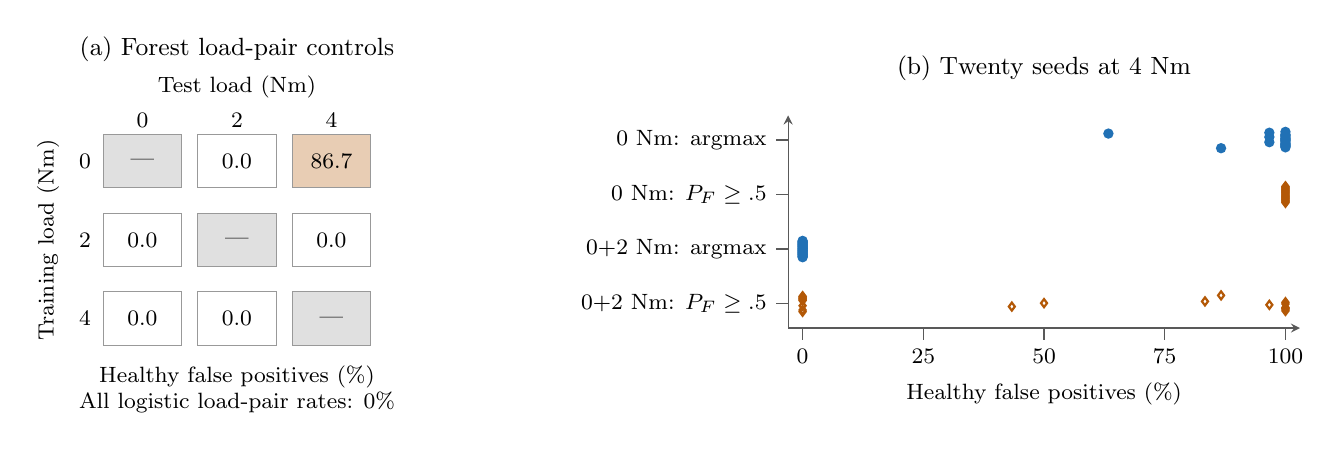
\begin{tikzpicture}[font=\footnotesize]
\tikzset{loadcell/.style={draw=black!40,minimum width=1.0cm,minimum height=.68cm}}
\node[font=\small] at (1.8,3.82) {(a) Forest load-pair controls};
\node at (1.8,3.34) {Test load (Nm)};
\node[rotate=90] at (-.6,1.4) {Training load (Nm)};
\node at (0.6,2.92) {0};
\node at (-.13,2.4) {0};
\node at (1.7999999999999998,2.92) {2};
\node at (-.13,1.4) {2};
\node at (3.0,2.92) {4};
\node at (-.13,0.3999999999999999) {4};
\node[loadcell,fill=black!12] at (0.6,2.4) {\textemdash};
\node[loadcell,fill=white] at (1.7999999999999998,2.4) {0.0};
\node[loadcell,fill=auditorange!30] at (3.0,2.4) {86.7};
\node[loadcell,fill=white] at (0.6,1.4) {0.0};
\node[loadcell,fill=black!12] at (1.7999999999999998,1.4) {\textemdash};
\node[loadcell,fill=white] at (3.0,1.4) {0.0};
\node[loadcell,fill=white] at (0.6,0.3999999999999999) {0.0};
\node[loadcell,fill=white] at (1.7999999999999998,0.3999999999999999) {0.0};
\node[loadcell,fill=black!12] at (3.0,0.3999999999999999) {\textemdash};
\node[align=center] at (1.8,-.50) {Healthy false positives (\%)\\All logistic load-pair rates: 0\%};
\begin{axis}[auditaxis,at={(8.8cm,.28cm)},anchor=south west,
width=6.5cm,height=2.7cm,xmin=-3,xmax=103,ymin=.55,ymax=4.45,
xtick={0,25,50,75,100},ytick={1,2,3,4},
yticklabels={{0+2 Nm: $P_F\geq.5$},{0+2 Nm: argmax},{0 Nm: $P_F\geq.5$},{0 Nm: argmax}},
xlabel={Healthy false positives (\%)},
title={(b) Twenty seeds at 4 Nm},
extra y ticks={},clip=false]
\addplot[only marks,color=auditblue,mark=*,mark size=1.45pt] coordinates {(86.666666666666686,3.8500000000000001) (100,3.8657894736842104) (100,3.8815789473684212) (100,3.8973684210526316) (100,3.9131578947368419) (100,3.9289473684210527) (100,3.9447368421052631) (96.666666666666686,3.9605263157894739) (100,3.9763157894736842) (100,3.9921052631578946) (100,4.007894736842105) (100,4.0236842105263158) (100,4.0394736842105265) (96.666666666666686,4.0552631578947365) (100,4.0710526315789473) (100,4.0868421052631581) (100,4.1026315789473689) (63.333333333333343,4.1184210526315788) (96.666666666666686,4.1342105263157896) (100,4.1500000000000004)};
\addplot[only marks,color=auditorange,mark=diamond,mark size=1.45pt] coordinates {(100,2.8500000000000001) (100,2.8657894736842104) (100,2.8815789473684212) (100,2.8973684210526316) (100,2.9131578947368419) (100,2.9289473684210527) (100,2.9447368421052631) (100,2.9605263157894739) (100,2.9763157894736842) (100,2.9921052631578946) (100,3.0078947368421054) (100,3.0236842105263158) (100,3.0394736842105265) (100,3.0552631578947369) (100,3.0710526315789473) (100,3.0868421052631581) (100,3.1026315789473684) (100,3.1184210526315788) (100,3.1342105263157896) (100,3.1499999999999999)};
\addplot[only marks,color=auditblue,mark=*,mark size=1.45pt] coordinates {(0,1.8500000000000001) (0,1.8657894736842104) (0,1.881578947368421) (0,1.8973684210526316) (0,1.9131578947368422) (0,1.9289473684210527) (0,1.9447368421052631) (0,1.9605263157894737) (0,1.9763157894736842) (0,1.9921052631578948) (0,2.0078947368421054) (0,2.0236842105263158) (0,2.0394736842105265) (0,2.0552631578947369) (0,2.0710526315789473) (0,2.0868421052631581) (0,2.1026315789473684) (0,2.1184210526315788) (0,2.1342105263157896) (0,2.1499999999999999)};
\addplot[only marks,color=auditorange,mark=diamond,mark size=1.45pt] coordinates {(0,0.84999999999999998) (100,0.86578947368421055) (0,0.88157894736842102) (100,0.89736842105263159) (100,0.91315789473684217) (100,0.92894736842105263) (43.333333333333336,0.94473684210526321) (0,0.96052631578947367) (96.666666666666671,0.97631578947368425) (100,0.99210526315789471) (50,1.0078947368421052) (100,1.0236842105263158) (83.333333333333343,1.0394736842105263) (0,1.0552631578947369) (0,1.0710526315789475) (0,1.0868421052631578) (0,1.1026315789473684) (0,1.118421052631579) (0,1.1342105263157896) (86.666666666666671,1.1499999999999999)};
\end{axis}
\end{tikzpicture}

\caption{\textbf{Measured healthy-row failure rates varied with training set and decision rule.} (a) Healthy false-positive rates for all six directed forest load pairs at the original seed; every logistic control was zero. Diagonal cells were not evaluated. (b) Each point denotes one of twenty forest seeds on the same 4-Nm normal recording; vertical jitter separates seeds. Labels specify source loads and the binary decision rule. Argmax collapses the three-class prediction; $P_F$ sums fault probabilities. Points are not independent-asset replicates or confidence intervals.}
\end{figure}
\clearpage
\end{document}
